\documentclass[a4paper, twoside]{report}

%% Language and font encodings
\usepackage[english]{babel}
\usepackage[utf8x]{inputenc}
\usepackage[T1]{fontenc}

%% Sets page size and margins
\usepackage[a4paper,top=3cm,bottom=2cm,left=3cm,right=3cm,marginparwidth=1.75cm]{geometry}

%% Useful packages
\usepackage{amsmath}
\usepackage{amssymb}
\usepackage{array}
\usepackage{graphicx}
\usepackage[colorinlistoftodos]{todonotes}
\usepackage[colorlinks=true, allcolors=black]{hyperref}
\usepackage{algorithm}
\usepackage{algpseudocode}
\usepackage{float}
\usepackage{underscore}
\usepackage{subfigure}

\newcolumntype{C}{>{$}c<{$}} % math-mode version of "l" column type

\title{Quasi-Monte Carlo methods for calculating derivatives sensitivities on the GPU}
\author{Casey Williams}
% Update supervisor and other title stuff in title/title.tex

\begin{document}
\begin{titlepage}

\newcommand{\HRule}{\rule{\linewidth}{0.5mm}} % Defines a new command for the horizontal lines, change thickness here

%----------------------------------------------------------------------------------------
%	LOGO SECTION
%----------------------------------------------------------------------------------------


\includegraphics[width=8cm]{title/logo.eps}\\[1cm] % Include a department/university logo - this will require the graphicx package
 
%----------------------------------------------------------------------------------------

\center % Center everything on the page

%----------------------------------------------------------------------------------------
%	HEADING SECTIONS
%----------------------------------------------------------------------------------------

\textsc{\LARGE BEng Individual Project Report}\\[1.5cm] % Name of your university/college
\textsc{\Large Imperial College London}\\[0.5cm] % Major heading such as course name
\textsc{\large Department of Computing}\\[0.5cm] % Minor heading such as course title

%----------------------------------------------------------------------------------------
%	TITLE SECTION
%----------------------------------------------------------------------------------------
\makeatletter
\HRule \\[0.4cm]
{ \huge \bfseries \@title}\\[0.4cm] % Title of your document
\HRule \\[1.5cm]
 
%----------------------------------------------------------------------------------------
%	AUTHOR SECTION
%----------------------------------------------------------------------------------------

\begin{minipage}{0.4\textwidth}
\begin{flushleft} \large
\emph{Author:}\\
\@author % Your name
\end{flushleft}
\end{minipage}
~
\begin{minipage}{0.4\textwidth}
\begin{flushright} \large
\emph{Supervisor:} \\
Dr. Paul A. Bilokon \\[1.2em] % Supervisor's Name
\emph{Second Marker:} \\
Dr. Maria Grazia Vigliotti % second marker's name
\end{flushright}
\end{minipage}\\[2cm]
\makeatother

% If you don't want a supervisor, uncomment the two lines below and remove the section above
%\Large \emph{Author:}\\
%John \textsc{Smith}\\[3cm] % Your name

%----------------------------------------------------------------------------------------
%	DATE SECTION
%----------------------------------------------------------------------------------------

{\large \today}\\[2cm] % Date, change the \today to a set date if you want to be precise

\vfill % Fill the rest of the page with whitespace

\end{titlepage}

\begin{abstract}
The calculation of option Greeks is vital for risk management. Traditional pathwise and finite-difference methods work poorly for higher-order Greeks and options with discontinuous payoff functions. The Quasi-Monte Carlo-based conditional pathwise method (QMC-CPW) for options Greeks allows the payoff function of options to be effectively smoothed allowing for increased efficiency when calculating sensitivities. Also demonstrated in literature is the increased computational speed gained by applying GPUs to highly parallelisable finance problems such as calculating Greeks. In this report QMC-CPW is paired with simulation on the GPU using the CUDA platform. We estimate the delta, vega and gamma Greeks of three exotic options: arithmetic Asian, binary Asian, and lookback. Not only are the benefits of QMC-CPW shown through variance reduction factors of up to $1.0 * 10^{18}$, but the increased computational speed through usage of the GPU is shown as we achieve speedups over sequential CPU implementations of more than $200$x for our most accurate method.
\end{abstract}


\renewcommand{\abstractname}{Acknowledgements}
\begin{abstract}
I would like to thank my supervisor Dr. Paul Bilokon for his support throughout this project.
\\
\\
I also wish to extend my thanks to Prof. Mike Giles of the University of Oxford for all of the help he has very kindly given.
\\
\\
Finally, thank you to the friends I have made over these past few years and to my family, for all the memories and support.
\end{abstract}

\tableofcontents 
\listoffigures
\listoftables
\listofalgorithms

\chapter{Introduction}

Calculating sensitivities (Greeks) of the value of an option to underlying parameters such as volatility and interest rates, is vital to financial institutions performing risk management and developing hedging strategies. Their importance becomes more significant when we know that Greeks cannot be observed in the market directly, thus must be calculated from other data.

Traditional finite-difference (FD) methods for calculating Greeks have easy implementations and few restrictions on the form of the payoff function, however they require resimulations which result in estimates with large variances, bias and increased computational effort compared with other methods. 

The pathwise (PW) \cite{glasserman1991gradient} method does not require resimulation and provides unbiased estimators, however it relies on the continuity of the payoff function, therefore it is not applicable to options such as a binary Asian option and cannot be used to calculate most second-order Greeks where we typically see discontinuity introduced into the function.

The likelihood ratio (LR) method does not require smoothness of the payoff function however it tends to result in estimates with large variance as it does not use properties of the payoff function.

Introduced by Zhang and Wang, the Quasi-Monte Carlo-based conditional pathwise method (QMC-CPW) \cite{ZhangConditionalQuasiMonteCarloMethod} takes a conditional expectation of the payoff function which results in the discontinuous integrand being smoothed. They also show that the interchange of expectation and differentiation is possible, allowing the estimation of Greeks from the now smooth target function. Through proof of the smoothed payoff being Lipschitz continuous, the PW method is now applicable to provide unbiased estimators. They also show how many options can have infinitely differentiable target functions once the conditional expectation is taken, thus the PW method can be used to calculate second-order Greeks which normally is not possible.

GPUs have been discussed extensively in literature. Particularly their application to finance problems. The highly parallel nature of Monte Carlo simulation for option Greeks lends itself well to the architecture of GPUs and the CUDA architecture. In this project we implement Monte Carlo methods which take advantage of the highly parallel nature of the GPU to gain advantages in speed and efficiency when calculating Greeks.

First, the preliminaries are discussed and the core mathematics of stochastic processes, financial products, and random number generation is developed in Chapter \ref{cha:Preliminaries}. Background literature on topics such as the usage of Monte Carlo and their implementation on GPUs, variance reduction techniques, and methods for estimating Greeks are discussed in Chapter \ref{cha:Background}. In Chapter \ref{cha:Implementation} we detail the implementation of our experiment on both the GPU and CPU, followed by the results in Chapter \ref{cha:Results}. We then evaluate the results and conclude in Chapters \ref{cha:Evaluation} and \ref{cha:Conclusion}.

\section{Objectives}
The aim of this work is to apply QMC-CPW to calculate Greeks for options, whilst adapting the implementation to run efficiently on a GPU.

Increased efficiency is not the only aim, but also the broadening of the set of financial products (such as those with discontinuous payoff functions) supported by the algorithm will provide further practical value. As opposed to other solutions developed for the GPU, we will produced unbiased estimates with low variance applicable to options with discontinuous payoff functions and for higher-order Greeks.

\section{Challenges}
Adapting algorithms to run on the GPU comes with many restrictions when compared to implementations on the CPU. Memory management and access patterns play a large role in the efficiency and speed when running kernels, so close attention must be paid during implementation to how the on-device memory is used.

CUDA poses further limitations upon the general design of the software such as having separate memory spaces between host and device memory (this has been addressed by unified memory which has been available since toolkit version 6.0). Problems such as these are standard when programming with CUDA and require overhead on the developer's side to ensure code is written in a safe manner.

\section{Contributions}
The work presented in the report is motivated by the importance of calculating Greeks for many financial institutions. The need for efficient and accurate methods that can be applied to many types of financial options presents an opportunity to use recent methods for Greeks estimation in conjunction with GPUs, and to obtain both an increase in accuracy and speed. The contributions are as follows:

\begin{enumerate}
    \item Flexible models of "products" are implemented for the arithmetic Asian, binary Asian and lookback option types. They have a templated design which allows for minimal reproduction of simulation kernels.
    \item GPU implementation of the Likelihood Ratio method for estimating Greeks which acts as a baseline to compare variance reduction factors of other methods. All methods estimate the \textit{delta}, \textit{vega}, and \textit{gamma} Greeks.
    \item Implementation of the QMC-CPW method with standard and Quasi Monte Carlo simulation on both CPU and GPU. CPU implementations are serial and used for comparison of the speedup obtained by using the GPU.
    \item For standard Monte Carlo simulations, antithetic variables are also implemented as a variance reduction technique.
    \item For Quasi-Monte Carlo we perform Brownian bridge construction which produces Brownian path increments for use in simulation of the behaviour of the underlying asset, which leads to a variance reduction.
    \item We show that the Quasi-Monte Carlo Conditional Pathwise method with Brownian bridge construction (QMC+BB-CPW) is the superior method in terms of accuracy with variance reduction factors of up to $1.0 * 10^{18}$ and with many in the hundreds of thousands and millions.
    \item We show that using the GPU leads to a massive speedup over the CPU with even the slowest methods being more than $200$x faster.
    \item Finally, it is shown that QMC+BB-CPW implemented on the GPU results in an efficient, accurate, and fast method for calculating first- and higher-order Greeks of options, and even those with discontinuous payoff functions. We find Quasi-Monte Carlo takes advantage of the increased smoothness in the integrand following the conditional expectation from CPW, and that the Brownian bridge construction results in further variance reduction.
\end{enumerate}
\chapter{Preliminaries} \label{cha:Preliminaries}
This chapter details the requisite material for understanding the approach and implementation.

First, an overview of basic financial products and models are presented, as well as some risk measures. We then detail the concepts behind one of the most popular approaches to computational finance problems - Monte Carlo methods. Later, common methods for calculating sensitivities of financial products with respect to input parameters are described. Lastly, we touch on the application of GPUs to related problems and outline the CUDA architecture and its toolkit, followed by a brief review of other literature.

\section{Stochastic processes}
A stochastic process is a collection of random variables indexed by time, or alternatively, a probability distribution of a space of paths. In the following subsections we describe some specific cases of stochastic processes.

\subsection{Brownian motion}
A \textit{standard} Brownian motion over $[0,T]$ is a stochastic process $\{W(t), 0 \le t \le T\}$ with the following properties \cite{glasserman2004monte}:

\begin{enumerate}
    \item $W(0) = 0$;
    \item the mapping $t \mapsto W(t)$ is, with probability $1$, a continuous function on $[0,T]$;
    \item the increments $\{ W(t_1) - W(t_0), W(t_2) - W(t_1),\dots,W(t_k) - W(t_{k-1})\}$ are independent for any $k$ and any $0 \le t_0 < t_1 < \dots < t_k \le T$;
    \item $W(t) - W(s) \sim N(0, t-s)$ for any $0 \le s < t \le T$.
\end{enumerate}

We can see from properties $1$ and $4$ that 

\begin{equation}
    W(t) \sim N(0,t),
\end{equation}

for $0 < t \le T$.

We may also construct a Brownian motion $X(t)$ with a constant \textit{drift} $\mu$ and \textit{diffusion coefficient} $\sigma > 0$ as

\begin{equation*}
    X(t) = \mu t + \sigma W(t),
\end{equation*}

where the following is a standard Brownian motion: 

\begin{equation*}
    \frac{X(t) - \mu t}{\sigma}.
\end{equation*}

In Figure \ref{fig:standardbrownianmotion} three example paths of standard Brownian motion are shown.

\begin{figure}[h]
    \centering
    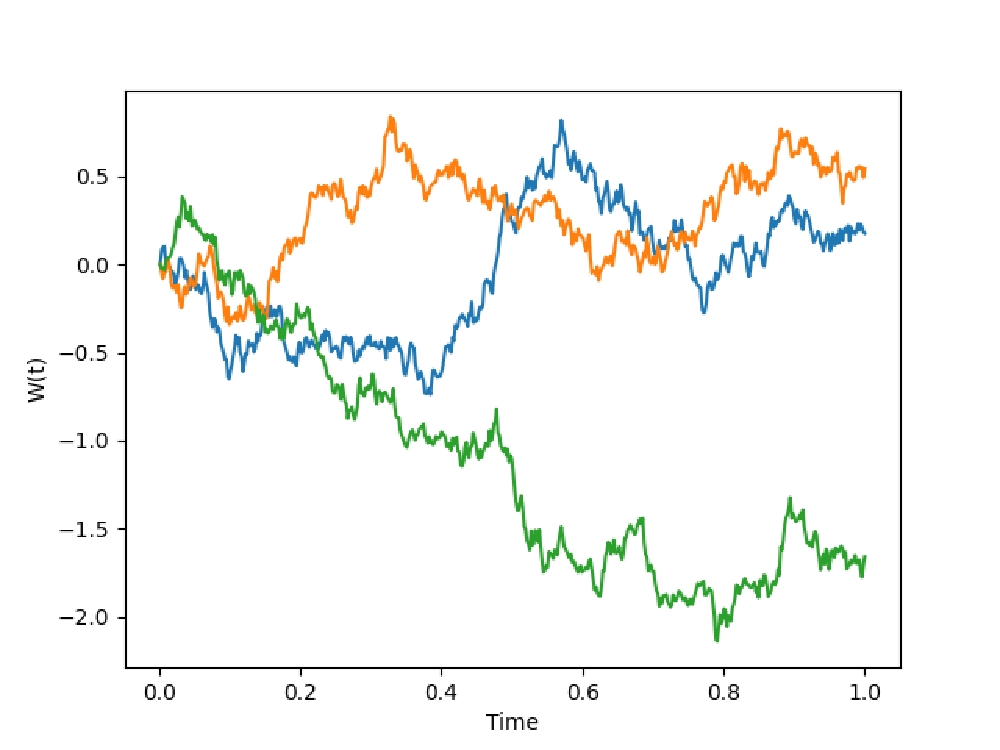
\includegraphics[width=0.8\textwidth]{figures/standard brownian motion.pdf}
    \caption{Three paths of a standard Brownian motion over $1$ year with $2^9$ equidistant timesteps.}
    \label{fig:standardbrownianmotion}
\end{figure}

\subsection{Martingales}
A stochastic process $X_t$ is known as a Martingale if 

\begin{equation*}
    E[X_t|\mathcal{F}_t] = X_s, \quad 0 \le s < t < \infty.
\end{equation*}

In other words, the conditional value of the next value in the sequence at any time $s$ is equal to the present value. If we use Martingales to model the price of an underlying asset, it means that all previous information about the price is available at the present time and we can disregard the past information. This fact, along with others, makes Martingales extremely useful in finance applications.

\section{Financial preliminaries}
\subsection{Derivatives}
Financial markets contain a wide range of products which are traded by market participants. One class of these products are known as \textit{derivatives}. A derivative is a contract whose value is derived from an asset, index, interest rate or other entity known as the "underlying". Derivatives are used for many purposes such as hedging risk or increasing exposure to underlying market changes and are ubiquitous in financial markets. Derivative contracts typically specify a set of conditions that define the obligations of the involved parties, important dates (such as expiration) and the notional value. Common types of derivatives are options, futures and swaps. 
Derivatives are of particular focus in computational finance as complex models which require high amounts of computation are needed to approximate their prices or sensitivities to input parameters.

\subsection{Options}
One of the most popular types of derivative is an option. An option is a contractual agreement which gives the owner, commonly referred to as the \textit{holder}, the right, but not the obligation, to buy or sell the underlying asset at a given price, the \textit{strike price} \(K\), on or before a specified expiration date \(T\). A European-style option only allows the holder to exercise the option at expiration time whereas an American-style option can be exercised at any time before expiration. For vanilla (simple) European-style options, a "call" option is one where the holder has the right to buy the underlying at expiration and a "put" allows them to sell the underlying at expiration.

According to the Black-Scholes model \cite{blackscholes}, the evolution of the stock price is described by the stochastic differential (SDE)

\begin{equation} \label{eqn:BlackScholesSDE}
    \frac{dS(t)}{S(t)} = r dt + \sigma dW(t),
\end{equation}

with \(W\) a standard Brownian motion. The parameters \(r\) and \(\sigma\) are the mean rate of return and volatility of the stock price respectively. $S(t)$ denotes the price of the underlying at time $t$. In the case where the mean rate of return is equal to the continuously compound interest rate \(r\) we are implicitly describing the \textit{risk-neutral} dynamics of the stock price. This idea is discussed extensively in literature and is core to the "fundamental theorem of asset pricing". The reader is referred to \cite{Dybvig2003} and Section 1.2.1 of \cite{glasserman2004monte} for further explanation.

The solution to the SDE in (\ref{eqn:BlackScholesSDE}) is

\begin{equation} \label{eqn:STsolution}
    S(T) = S(0)\exp{([r - \frac{1}{2}\sigma^2]T + \sigma W(T))}.
\end{equation}

With \(S(0)\) known, and the current price of the stock. If now is time \(t=0\) and at expiration time \(T\) the price of the underlying \(S(T)\) is greater than the strike price \(K\) then the holder exercises the option for a profit of \(S(T) - K\). Conversely, if the terminal price \(S(T)\) is less than \(K\) then the option expires worthless. Thus the payoff to the holder at expiration is given as

\begin{equation} \label{eqn:EuropeanCallPayoff}
    (S(T) - K)^+ = \max{\{0, S(T) - K\}}.
\end{equation}

There exist more complex options whose values are path-dependant and others with payoff functions that are not continuous. These properties pose extra challenges from an implementation perspective and continue to be a focal point in current literature.

\section{Monte Carlo methods} \label{sec:MonteCarloMethods}
\subsection{Principles of Monte Carlo} \label{sec:MonteCarloPriciples}
Monte Carlo methods, in the simplest form, rely on repeatedly taking random samples from a set of possible outcomes to determine the fraction of random draws which fall in a given set as an estimate of the set's volume in the probability space \cite{glasserman2004monte}. As the number of draws increases, the law of large numbers ensures the estimate converges to the true value and information about the magnitude of error in the estimate can be obtained through the central limit theorem.

Let us use the example from Section 1.1.2 of \cite{glasserman2004monte}, suppose we wish to calculate the expected present value of the payoff of a vanilla European call option on a stock. The payoff for this option is defined in (\ref{eqn:EuropeanCallPayoff}). Taking \(S(t)\) to be modelled as in (\ref{eqn:BlackScholesSDE}) thus giving the terminal price in (\ref{eqn:STsolution}), we can then draw samples from the distribution of the terminal stock price \(S(T)\) to calculate the expected value of the payoff \(E[e^{-rT}(S(T) - K)^+]\). As \(W(t)\) is a standard Brownian motion, the logarithm of the stock price is normally distributed. Thus we only need to draw random samples \(Z_i\) from the standard normal distribution to calculate \(S(T)\). Pseudocode is given below for estimating the expected present value of the payoff on the call option:

\begin{algorithm}[hbt!]
\caption{Algorithm to estimate expected present value of payoff}\label{alg:EstimateExpectedPayoff}
\begin{algorithmic}[1]
\For{$i \gets 1..n$}
    \State generate $Z_i$
    \State $S_i(T) = S(0)\exp{([r - \frac{1}{2}\sigma^2]T + \sigma \sqrt{T}Z_i)}$
    \State $C_i = e^{-rT}(S_i(T) - K)^+$
\EndFor
\State $\hat{C_n} = (C_1 + \dots + C_n) / n$
\end{algorithmic}
\end{algorithm}

This method can be generalised to calculate payoffs for more exotic path-dependent options and to other problems such as calculating the Greeks of a portfolio of derivatives - see \cite{giles2007monte} for further explanation.

\subsection{Pseudorandom number generation} \label{sec:prng}
Randomly sampling from probability distributions is the heart of Monte Carlo, so generating random samples quickly with sufficient "randomness" has been the topic of much research. The core of generating random samples in Monte Carlo is a \textit{pseudorandom number generator} (PRNG). PRNGs are deterministic algorithms that generate sequences of numbers whose properties mimic that of genuine random sequences. We do not attempt to cover PRNGs extensively; for a more detailed review of PRNG algorithms and their properties the reader is referred to \cite{l2010pseudorandom}, \cite{gu2016statistical} and Chapter 2 of \cite{glasserman2004monte}.
Most PRNGs used for Monte Carlo simulation are based on linear recurrences of the form

\begin{equation*}
    x_i = (a_1 x_{i-1} + \dots + a_k x_{i-k}) \mod{m},
\end{equation*}

where $k$ and $m$ are positive integers with $a_1 \dots a_k$ in $\{0, 1, \dots , m-1\}$ and $a_k \neq 0$. $m$ is typically a large prime number and the output is defined as $u_i = x_i / m$. The \textit{seed} of a generator is the initial set of values $x_{k-1}, \dots, x_0$.

There are several considerations which we take into mind when building PRNGs:
\begin{itemize}
    \item \textit{Good randomness properties}. A sequence of genuine random numbers $U_1, U_2, \dots$ satisfy the following properties:
    \begin{enumerate}
        \item Each $U_i$ is uniformly distributed between 0 and 1 (this is an arbitrary normalisation, any other range is acceptable).
        \item All $U_i$ are mutually independent.
    \end{enumerate}
    This is the hardest property to ensure for PRNGs but there has been enough examination of generators over time and those that are still in use today typically have passed statistical tests which show little deviation from truly random sequences.
    \item \textit{Large period}. The period of a PRNG is the minimum length of the output sequence before any number is repeated. Generators with large periods are key for use in simulation as we wish to draw millions of samples and without a sufficiently large period this would not be possible.
    \item \textit{Speed and efficiency of generation}. As we are generating millions of samples during a single simulation it is necessary for this process to be fast and require little effort computationally.
    \item \textit{Reproducibility}. It is important that using the same seed will result in the same output sequence. This allows us to run simulations multiple times with the same input to verify results.
\end{itemize}

\section{Quasi-Monte Carlo} \label{sec:quasimc}
Whereas Monte Carlo methods use pseudorandom sequences, Quasi-Monte Carlo (QMC) uses \textit{low-discrepancy sequences} (LDS). Rather than mimic randomness, LDS attempt to generate numbers that are evenly distributed. The advantage of using LDS is the rate at which they converge; Monte Carlo converges with rate $O(1/\sqrt{n})$, where $n$ is the number of paths, while QMC has convergence rate close to $O(1/n)$. 

The reliance on LDS however, leads QMC to have a dependence on the dimension of the problem and with many financial problems having high dimension due to large numbers of risk factors, time steps per path and the number of paths simulated, it is not guaranteed that QMC has greater performance over Monte Carlo. This has been addressed through a number of techniques such as \textit{variance reduction} \cite{allen2011variance}, \cite{WANGvariancereduction} and the concept of \textit{effective dimension} \cite{caflisch_1998}, \cite{WANGeffectivedim} may explain the success of QMC even for problems of high dimension.

To highlight the difference between QMC and Monte Carlo, let us consider the problem of numerical integration over the unit hypercube $[0, 1)^d$. We want to calculate

\begin{equation} \label{eqn:UnitHypercubeIntegral}
    E[f(U_1, \dots, U_d)] = \int_{[0,1)^d} f(x) dx,
\end{equation}

where $U_i$ are uniformly distributed random variables. This integral is approximated by

\begin{equation} \label{eqn:ApproxUnitHypercubeIntegral}
    \int_{[0,1)^d} f(x) dx \approx \frac{1}{n} \sum_{i = 1}^n{f(x_i)}.
\end{equation}

To calculate this value using Monte Carlo, we can construct a sequence $U_1, U_2, \dots$ and form vectors $(U_1, \dots, U_d), (U_{d+1}, \dots, U_{2d}), \dots$ which represents an i.i.d. sequence of points uniformly distributed on the unit hypercube. Here, we do not depend on the dimension $d$ to generate the sequence whereas the construction of points for QMC depends explicitly on the dimension, thus we cannot generate vectors of $d$ elements repeatedly. Rather we use LDS to choose points that effectively "fill" the hypercube as uniformly as possible. Common LDS include Sobol' sequences \cite{sobol1967distribution} and Halton sequences \cite{haltonsequences}.

\subsection{Van der Corput sequences} \label{sec:VanDerCorputSequences}
To talk in further detail about Sobol' sequences, we must introduce Van der Corput sequences. Following \cite{glasserman2004monte}, this sequence is a specific class of LDS in one dimension and is the core of many multidimensional constructions.

Every positive integer $k$ has what is known as it's base-$b$ representation such that

\begin{equation} \label{eqn:BaseBKRepresentation}
    k = \sum_{j=0}^{\infty}{a_j(k)b^j},
\end{equation}

where $b \ge 2$ and finitely many of the coefficients $a_j(k)$ are not equal to zero and in $\{0,1\dots,b-1\}$. The \textit{radical inverse function} $\psi_b$ is a mapping of each $k$ to $[0,1)$ and is given as

\begin{equation} \label{eqn:RadicalInverseFunction}
    \psi_b(k) = \sum_{j=0}^{\infty}{\frac{a_j(k)}{b^{j+1}}}.
\end{equation}

The Van der Corput sequence in base-$b$ is $0 = \psi_b(0), \psi_b(1), \psi_b(2),\dots$ and we give the sequence in base $2$ below.

\begin{table}[!h]
\centering
$\begin{array}{ c c c c } 
 \hline
 k & k\;\text{Binary} & \psi_2(k)\;\text{Binary} & \psi_2(k) \\
 \hline
 0 & 0   & 0     & 0 \\
 1 & 1   & 0.1   & 1/2 \\
 2 & 10  & 0.01  & 1/4 \\
 3 & 11  & 0.11  & 3/4 \\
 4 & 100 & 0.001 & 1/8 \\
 5 & 101 & 0.101 & 5/8 \\
\end{array}$
\caption{Radical inverse function $\psi_b$ in base $2$.}
\label{tbl:RadicalInverseBase2}
\end{table}

Table \ref{tbl:RadicalInverseBase2} shows how the sequence fills the unit interval; the $k$th row shows the first $k$ nonzero elements of the sequence and each row refines the previous one. The Van der Corput sequence also fills the points in a maximally balanced way. For example following the final row of Table \ref{tbl:RadicalInverseBase2} we would fill $1/16$, then $9/16$, then $5/16$ and so on. The values alternate either side of $1/2$, then either side of $1/4$ and this continues. An important property to note is that the larger the base $b$, the greater the number of points required to reach uniformity.

\subsection{Sobol' sequences} \label{sec:SobolSequences}
First introduced by Sobol' in 1967 \cite{sobol1967distribution}, was the construction of a $(t,d)$-sequence. Sobol's construction can be contrasted with other LDS such as Faure's \cite{Faure1982} as Faure's points are $(0,d)$-sequences in a base at least as large as $d$ whereas Sobol's points are $(t,d)$-sequences in base $2$ for all $d$, with values of $t$ that depend on $d$ \cite{glasserman2004monte}. This gives Sobol' points the advantage of a much smaller base but with slightly less uniformity. The ability to work in base $2$ has obvious advantages when applied to the computational setting with bit-level operations.

The Sobol' points start from the Van der Corput sequence in base $2$ only and the coordinates of a $d$-dimensional sequence come from permutations of sections of the Van der Corput sequence. These permutations result from the product of binary expansions of consecutive integers with a set of generator matrices, one for each dimension. A generator matrix $\boldsymbol{G}$ has columns of binary expansions of a set \textit{direction numbers} $g_1,\dots,g_r$ with elements equal to $0$ or $1$. The value $r$ represents the number of terms in the binary expansion of $k$ and can be arbitrarily large. Let $(a_0(k),\dots,a_{r-1}(k))^\top$ represent the vector of coefficients of the binary representation of $k$ such that

\begin{equation} \label{eqn:GeneratorMatrixExpression}
    \begin{pmatrix}
    y_1(k) \\
    y_2(k) \\
    \vdots \\
    y_r(k)
    \end{pmatrix}
    = \boldsymbol{G} 
    \begin{pmatrix}
    a_0(k) \\
    a_1(k) \\
    \vdots \\
    a_{r-1}(k)
    \end{pmatrix}
    \mod{2},
\end{equation}

and $y_1(k),\dots,y_r(k)$ are the coefficients of the binary expansion of the $k$th point in the sequence. This gives the $k$th point as:

\begin{equation*}
    x_k = \frac{y_1(k)}{2} + \frac{y_2(k)}{4} + \dots + \frac{y_r(k)}{2^r}.
\end{equation*}

The generator matrix $\boldsymbol{G}$ is upper triangular and the special case where it is the identity matrix results in the Van der Corput sequence in base $2$. We can perform (\ref{eqn:GeneratorMatrixExpression}) in a computer implementation through a bitwise XOR operation, giving us the computer representation of $x_k$ as

\begin{equation*}
    a_0(k)g_1 \oplus a_1(k)g_2 \oplus \dots \oplus a_{r-1}(k)g_r,
\end{equation*}

where $\oplus$ is the bitwise XOR operator.

The core of the Sobol' method are the generator matrices $\boldsymbol{G}$ and their direction numbers $g_j$. As previously mentioned, we require $d$ sets of direction numbers to produce a $d$-dimensional sequence. The method begins by selecting a \textit{primitive polynomial} over binary arithmetic. The polynomial

\begin{equation} \label{eqn:SobolPrimitivePolynomial}
    x^q + c_1x^{q-1} + \dots + c_{q-1}x + 1,
\end{equation}

has coefficients $c_i$ in $\{0,1\}$ and satisfies two properties \cite{glasserman2004monte}:

\begin{itemize}
    \item it cannot be factored;
    \item the smallest power $p$ for which the polynomial divides $x^p + 1$ is $p = 2^q - 1$.
\end{itemize}

The primitive polynomial in (\ref{eqn:SobolPrimitivePolynomial}) defines a recurrence relation

\begin{equation} \label{eqn:SobolRecurrenceRelation}
    m_j = 2c_1m_{j-1} \oplus 2^2c_2m_{j-2} \oplus \dots \oplus 2^{q-1}c_{q-1}m_{j-q+1} \oplus 2^qm_{j-q} \oplus m_{j-q},
\end{equation}

where the $m_j$ are integers. We define the directions numbers as

\begin{equation*}
    g_j = \frac{m_j}{2^j}.
\end{equation*}

Of course, to fully define the direction numbers we need initial values for $m_1,\dots,m_q$. It is enough to set each initialising $m_j$ to be an odd integer less than $2^j$, which ensures that all following $m_j$ as defined by (\ref{eqn:SobolRecurrenceRelation}) also share this property. From this, each $g_j$ will be strictly between $0$ and $1$.

So, to construct a sequence we take the primitive polynomial and use the recurrence relation (\ref{eqn:SobolRecurrenceRelation}) with some initial $m_j$. We then calculate the corresponding direction numbers $g_j$ by dividing by $2^j$ (or performing a binary shift of the binary point $j$ places to the left). Then with these direction numbers we construct the generator matrix $G$. With this generator matrix we take a vector $\boldsymbol{a}(k)$ of binary coefficients of $k$ and perform the operation in (\ref{eqn:GeneratorMatrixExpression}) to give us the coefficients of a binary fraction, from which we obtain $x_k$.

There has been much research on choosing initial direction numbers, and also more efficient construction implementation (namely Gray code construction \cite{GrayCodeConstruction}), which we will not go into further detail about.

\subsection{Scrambled Sobol'} \label{sec:ScrambledSobol}
As we are choosing points deterministically we are unable to measure error through a confidence interval. In sacrificing some of the accuracy obtained through careful selection of points, randomised QMC points allow us to calculate this error. One method for producing randomised QMC points is known as \textit{scrambling}.

Introduced by Owen and further developed in \cite{OwenScrambling}, scrambling is a technique that permutes each digit of a $b$-ary expansion, where the permutation applied to the $j$th digit is dependent on the preceding $j-1$ digits. Scrambling can be described by taking each coordinate, partitioning the unit interval into $b$ subintervals of length $1/b$ and then randomly permuting those subintervals. Then, further partition each subinterval into $b$ subintervals of length $1/b^2$ and permute those, and so on. At the $j$th step, we have $b^{j-1}$ partitions, each of which consist of $b$ intervals, and each is permuted randomly and independently.

\section{Graphics Processing Units and CUDA}
The Graphics Processing Unit (GPU) has seen widespread adoption in computational finance due to its highly parallel architecture designed for increased computational throughput. When NVIDIA released CUDA \cite{cudazone} in 2007 it enabled more "general-purpose" usage of the previously graphics-focused applications of GPUs.

\subsection{CUDA architecture} \label{sec:cudaarch}
The CUDA architecture allows each and every arithmetic logic unit (ALU) on the chip to be marshaled by a program \cite{sanders2010cuda}. It is implemented by organising the the GPU into a collection of \textit{streaming multiprocessors}, which operate following the Single-Instruction-Multiple-Thread (SIMT) paradigm. Because of the intended usage for general-purpose computation CUDA allows for arbitrary read and write access to memory and the software-managed cache known as \textit{shared memory}.

From a software perspective, the CUDA architecture allows for \textit{kernels} to be ran in parallel across a \textit{grid}. This grid is composed of multiple \textit{blocks}, each of which contains a collection of threads which all run the program defined by some launched kernel. Both blocks and grids can have up to three dimensions each and CUDA provides useful syntax for indexing into them. In hardware, the threads inside of a block are grouped into sets of 32 threads known as a \textit{warp}, where all threads inside the same warp execute the same instruction.

\begin{figure}[h]
    \centering
    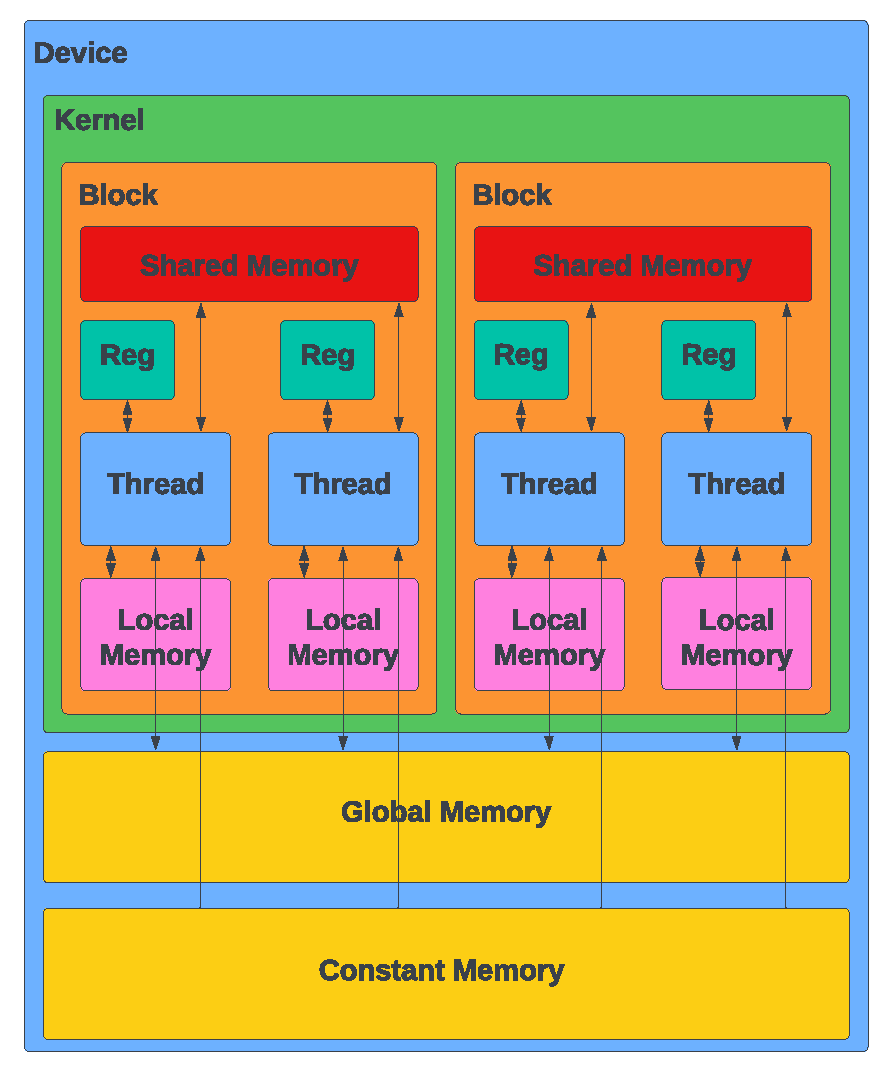
\includegraphics[width=0.6\textwidth]{figures/cuda arch.pdf}
    \caption{Basic CUDA memory architecture. Inspired by https://cvw.cac.cornell.edu/gpu/memory\_arch}
    \label{fig:cudaarch}
\end{figure}

Each thread has its own local memory and registers, and threads in the same block have access to the on-chip shared memory of that block. This is often how threads within a block communicate with each other while maintaining high performance. The basic architecture is shown in Figure \ref{fig:cudaarch}.

NVIDIA have also developed a toolkit for CUDA \cite{cudatoolkitdocumentation} which contains the compiler, highly parallel implementations of mathematical libraries (such as cuBLAS, cuRAND and cuFFT) and a host of other useful tools like a debugger and memory checker.

\subsection{Practical implementation considerations}
There are many considerations one must take into account when implementing algorithms on a GPU. Most notably, the limited size of on-chip caches in comparison to the relatively large size of global memory. For financial problems with high dimensions (such as Monte Carlo simulations of many paths or many assets) shared memory will quickly become a limiting factor to the speed of an implementation. This is because reading from global memory is roughly 100x slower than loading directly from shared memory. This limitation has been addressed in literature and a few common design patterns have arisen such as pre-computation of values shared between threads, merging of kernels to avoid redundant data transfers and using coalesced reads and writes. See \cite{dixon2012monte} for an example of how problem reformation can lead to large speed ups and see \cite{BrodtkorbGPU} for further discussion of GPU programming strategies.
\chapter{Background} \label{cha:Background}
This chapter provides an overview of developments in computational finance and the areas with which this project focuses on.

\section{Calculating Greeks}
Calculating price sensitivities (Greeks) is arguably more important than prices themselves. This is due to the use of Greeks for risk management and hedging. The calculation of Greeks requires significant computational effort when compared to that of determining derivative prices thus efficient implementation of algorithms for obtaining sensitivities is key for financial institutions.

\subsection{Finite-difference method}
The simplest method for obtaining sensitivities is based on the finite-difference approach. Within the Monte Carlo framework this involves running multiple simulations of a pricing routine over a range of values of input parameters. For example, determining the delta of a call option would involve running simulations for different values of the underlying price and observing the changes in the resulting option price. To obtain the derivative of an options price with respect to input parameter $\theta$ we would estimate 

\begin{equation*}
    \frac{\partial V(t, \theta)}{\partial \theta} \approx \frac{V(t, \theta + h) - V(t, \theta)}{h},
\end{equation*}

where $V(t, \theta)$ is the value of the payoff of the option at time $t$ and some small $h \in \mathbb{R}^+$ known as the "bump size".

The finite-difference method is intuitive and easy to implement, however it requires significantly higher computation time as the number of input parameters grows and suffers from poor bias and variance properties.

\subsection{Pathwise method} \label{sec:PathwiseMethod}
An alternative to finite-difference is the pathwise method. Developed by Glasserman \cite{glasserman1991gradient} and explained further by Broadie and Glasserman \cite{broadie1996estimating}, the pathwise method has two main benefits: increased computational speed and unbiased estimates. To explain the pathwise method, let us consider the calculation of the delta of a vanilla European call option on a stock that satisfies (\ref{eqn:BlackScholesSDE}). Let $Y$ denote the present value of the payoff

\begin{equation*}
    Y = e^{-rT}[S(T) - K]^+.
\end{equation*}

Applying the chain rule we obtain

\begin{equation} \label{eqn:ChainRuleOptionDelta}
    \frac{\partial Y}{\partial S(0)} = \frac{\partial Y}{\partial S(T)} \frac{\partial S(T)}{\partial S(0)}.
\end{equation}

Observe that (\ref{eqn:STsolution}) is linear in $S(0)$ and so $\partial S(T)/ \partial S(0) = S(T)/S(0)$. We have $\partial Y/ \partial S(T) = e^{-rT}\textbf{1}\{S(T) > K\}$, combining the two gives us the pathwise estimator for the delta

\begin{equation} \label{eqn:PathwiseDeltaEstimate}
    \frac{\partial Y}{\partial S(0)} = e^{-rT} \frac{S(T)}{S(0)} \textbf{1}\{S(T) > K\}.
\end{equation}

We can obtain other first-order and higher-order derivatives through similar means. It can be seen that (\ref{eqn:PathwiseDeltaEstimate}) is easily evaluated and has been shown to be an unbiased estimator \cite{broadie1996estimating}. The method can also be applied to path-dependent options and provides a lot of practical value for options with no closed-form solution (such as Asian options). Further, as many of the factors used in calculating an options price are present in the pathwise estimators, little effort is required to add them to an existing pricing implementation.

To provide context of how pathwise is used within Monte Carlo, let us consider calculating the delta of a derivative security with multiple underlying assets and payoff function $f$. We model the evolution of a stock price such that it satisfies a similar SDE to (\ref{eqn:BlackScholesSDE}) but where $W$ is a $d$-dimensional Brownian motion, and we are approximating the price using a Euler scheme with timestep $h = T/N$, we can write the Euler approximation at time $nh$ as follows:

\begin{equation} \label{eqn:EulerApproximation}
    \hat{S}(n + 1) = \hat{S}(n) + a(\hat{S}(n))h + b(\hat{S}(n)) Z(n+1) \sqrt{h}, \quad \hat{S}(0) = S(0), 
\end{equation}

with $a(\cdot) \in \mathbb{R}^m$, $b(\cdot) \in \mathbb{R}^{m \times d}$ and $Z(1), Z(2), \dots$ are $d$-dimensional standard normal random vectors. (\ref{eqn:EulerApproximation}) then takes the form

\begin{equation} \label{eqn:EulerMatrixForm}
    \hat{S}(n + 1) = F_n(\hat{S}(n)),
\end{equation}

with $F_n$ a matrix transformation $\mathbb{R}^m \to \mathbb{R}^m$. Then we can perform similar operations as in (\ref{eqn:ChainRuleOptionDelta}), we obtain the pathwise estimate of the delta

\begin{equation} \label{eqn:MatrixPathwiseDeltaEstimate}
    \sum_{i=1}^m \frac{\partial f(\hat{S}(N)}{\partial \hat{S}_i(N)} \Delta_{ij}(N)
\end{equation}

with

\begin{equation*}
    \Delta_{ij}(n) = \frac{\partial \hat{S}_i(n)}{\partial \hat{S}_j(0)}, \quad i,j = 1, \dots, m.
\end{equation*}

This can be written as a matrix recursion

\begin{equation} \label{eqn:DeltaMatrixRecursion}
    \Delta (n + 1) = G(n) \Delta (n), \quad \Delta (0) = I,
\end{equation}

where $G(n)$ represents the derivative of the transformation $F_n$ and $\Delta (n)$ is the $m \times m$ matrix with entries $\Delta_{ij}(n)$.

There are some limitations to the pathwise method, namely the payoff function must be Lipschitz continuous but there exist other methods to overcome this problem such as smoothing the payoff function, using the Likelihood Ratio Method (LRM) (see \ref{sec:LikelihoodRatioMethod}) or an alternative form of Monte Carlo simulation such as "Vibrato" Monte Carlo \cite{giles2009vibrato}.

\subsection{Likelihood ratio method} \label{sec:LikelihoodRatioMethod}
Rather than view the final state of a stock price as a random variable, as in (\ref{eqn:STsolution}), we can look from the perspective of a probability distribution \cite{broadie1996estimating}. For an option with payoff function $Y = f(S(T))$ and underlying satisfying (\ref{eqn:BlackScholesSDE}) such that the payoff is expressed as a function of a random vector $X = (X_1,\dots,X_d)$, its value can be written as

\begin{equation} \label{eqn:OptionValueProbabilityForm}
    V = E[f(Y)] = \int f(x) g_\theta (x) dx,
\end{equation}

where $g_\theta$ is probability density function of $X$. Supposing that the interchange of order between integration and differentiation holds, we can take the derivative of (\ref{eqn:OptionValueProbabilityForm}) with respect to an input parameter $\theta$ to obtain the likelihood ratio estimator

\begin{equation} \label{eqn:LRUnbiasedEstimate}
    \frac{\partial V}{\partial \theta} = \int f(x) \frac{g^\prime_\theta(x)}{g_\theta(x)} g_\theta(x)dx = E\left[f(X) \frac{g^\prime_\theta(X)}{g_\theta(X)} \right].
\end{equation}

As probability densities are generally continuous we can apply the LRM to calculate Greeks for derivatives with discontinuous payoff functions and, as with the pathwise method, it works well for path-dependent options.

A weakness of LRM lies in its $O(h^{-1})$ estimator variance where $h$ is the timestep for the path discretisation in simulation.

\section{Monte Carlo methods}
Monte Carlo simulation is an essential tool in computational finance for calculating prices of derivatives and their sensitivities to input parameters, commonly known as the "Greeks". The application of Monte Carlo simulation to pricing derivatives was first developed by Boyle in 1977 \cite{BOYLE1977323} and has shown to be an efficient method for high-dimensional problems. The ease of implementation and intuitiveness behind Monte Carlo have continued to make it a key approach for many problems in computational finance \cite{glasserman2004monte}.

Following Boyle's seminal paper, application of Monte Carlo methods to many problems in finance and the acceleration of implementations became a focus in literature. For a review of early Monte Carlo methods and their use for calculating derivatives prices see \cite{boyle1997monte}.

Broadie and Glasserman \cite{broadie1996estimating} develop two techniques which allow for increased computational speed over the traditional finite-difference method when calculating derivative sensitivities through Monte Carlo simulation. The basics of these two methods are detailed in \ref{sec:PathwiseMethod} and \ref{sec:LikelihoodRatioMethod}. These "direct methods" not only speed up simulation but provide \textit{unbiased estimators} for sensitivities, unlike finite-difference, and work for path-dependant options.

The issue of discontinuous payoff functions has been discussed extensively in literature and still continues to be a popular topic. Giles presents the "Vibrato" Monte Carlo method \cite{giles2009vibrato} which combines the adjoint pathwise approach for the stochastic path evolution, with the likelihood ratio method (LRM) for evaluation of the payoff function. He shows that when the payoff function is discontinuous the resulting estimator has variance $O(h^{-1/2})$, where $h$ is the timestep for the path discretisation, and $O(1)$ when the payoff is continuous. The numerical results presented show its superior efficiency when compared to standard LRM.

\subsection{GPU implementations}
There are several properties of Monte Carlo which make it attractive for an implementation with high parallelism, thus in recent years much work has been done on using GPUs to accelerate these simulations.

Dixon et al. \cite{dixon2012monte} show that Monte Carlo is well suited to implementation on a high performance GPU and discuss methods for accelerating Value-at-Risk estimation through several key implementation techniques. More recently, the techniques discussed in \ref{sec:PathwiseMethod} paired with Algorithmic Adjoint Differentiation (AAD) have also seen implementation on the GPU \cite{savickas2014super} and have shown speed-ups of over 10 times when compared to traditional finite difference methods on GPUs, and more than 70 times when compared to multi-core CPU implementations.

\section{Variance reduction techniques}
Boyle et al. \cite{boyle1997monte} discuss variance reduction techniques and show that their application reduces the error in estimates, thus increasing the efficiency of Monte Carlo simulation. In its simplest form, the argument for variance reduction techniques to increase \textit{efficiency}. If we have two (unbiased) Monte Carlo estimates for parameter $\theta$, denoted by $\{ \hat{\theta}_i^{(1)}, i = 1, 2, \dots \}$ and $\{ \hat{\theta}_i^{(2)}, i = 1, 2, \dots \}$, with $b^{(j)}, j = 1, 2$, the computational work required to generate one replication of $\hat{\theta}^{(j)}$, then we would choose estimator $1$ over $2$ if

\begin{equation} \label{eqn:EstimatorEfficiencyComparison}
    \sigma_1^2 b_1 < \sigma_2^2 b_2,
\end{equation}

where $\sigma_j^2$ is the variance of the estimator $\hat{\theta}^{(j)}$. We can take the product of variance and computational work to be a measure of the efficiency, thus use (\ref{eqn:EstimatorEfficiencyComparison}) as a way to compare multiple Monte Carlo estimators. We briefly detail some of the common techniques to reduce variance in the following sections. For further explanation, the reader is referred to \cite{glasserman2004monte} and \cite{boyle1997monte}.

\subsection{Antithetic variables} \label{sec:antitheticvariables}
The idea behind antithetic variables comes from the fact that if $Z_i$ has standard normal distribution, then $-Z_i$ also does. Therefore, if we have generated a sample path from inputs $Z_1, \dots, Z_n$ we can generate a second path $-Z_1, \dots, -Z_n$. The variables $Z_i$ and $-Z_i$ form an \textit{antithetic pair} such that a large value in an estimate obtained from $Z_i$ will be paired with a small value obtained from $-Z_i$.

As an example, let $C$ denote the value of a vanilla European call option. We have an existing unbiased estimate $C_i$ generated as in line 4 of Algorithm \ref{alg:EstimateExpectedPayoff} in \ref{sec:MonteCarloPriciples}. From the idea described above, we can generate a second unbiased estimate $\tilde{C_i}$, from a sample terminal stock price using $-Z_i$. Therefore, we can take

\begin{equation*}
    \hat{C}_{AV} = \frac{1}{n} \sum_{i=1}^n \frac{C_i + \tilde{C_i}}{2}
\end{equation*}

as an unbiased estimator for the call price. Heuristically, estimates obtained from $n$ antithetic pairs ${Z_i, -Z_i}$ are distributed more regularly than a collection of $2n$ independent samples, thus may reduce variance. It can be shown that the requirements to increase efficiency when calculating $\hat{C}_{AV}$ are easily satisfied for estimators of options that depend monotonically on inputs (e.g. European and Asian options) \cite{boyle1997monte}.

\subsection{Control variates}
Control variates use the idea that exploiting errors in estimates of \textit{known} quantities, allows you to evaluate an estimate for an \textit{unknown} quantity through their difference.

Suppose we have the unbiased estimate $\hat{X}$ for the unknown expectation $X = E[\hat{X}]$, from a single simulated path. We can also calculate another output $\hat{Y}$ where the expectation $Y = E[\hat{Y}]$ is known. We can write

\begin{equation*}
    X = Y + E[\hat{X} - \hat{Y}].
\end{equation*}

Simply, $X$ can be expressed as the known value $Y$ plus the expected difference. This provides the unbiased estimator

\begin{equation*}
    \hat{X}_{CV} = \hat{X} + (Y - \hat{Y}),
\end{equation*}

where the observed error $(Y - \hat{Y})$ is the \textit{control} in the estimation of $X$.

It is shown that the estimator $\hat{X}_{CV}$ has smaller variance than the estimator $\hat{X}$ when the correlation between $X$ and $Y$ is large \cite{boyle1997monte}. Given that little additional effort is required to calculate the control variate, the method provides good computational speed up when the previous condition holds.

\subsection{Importance sampling}
Importance sampling uses the idea that expectations from two probability measures can be expressed in terms of each other, and by switching measure we can reduce variance. The change of measure is used to give more weight to "important" results in order to obtain a more efficient estimator.

Consider the problem of estimating

\begin{equation*}
    \alpha = E[f(X)] = \int f(x) p(x) dx,
\end{equation*}

where $X \in \mathbb{R}^d$ is a random variable with probability density $p$ and $f$ is some function $\mathbb{R}^d \to \mathbb{R}$. The Monte Carlo estimate 

\begin{equation*}
    \hat{\alpha} = \frac{1}{n} \sum_{i=1}^n f(X_i)
\end{equation*}

with $X_i$ i.i.d random samples from $p$. Through change of measure we can rewrite our estimate as

\begin{equation*}
    \hat{\alpha}_q = \frac{1}{n} \sum_{i=1}^n f(X_i) \frac{p(X_i)}{q(X_i)},
\end{equation*}

with $q$ as some other probability density satisfying $p(x) > 0 \Rightarrow q(x) > 0$. The value $p(X_i)/q(X_i)$ is known as the \textit{likelihood ratio} and through careful selection of the importance sampling distribution $q$, we can obtain estimates with lower variance than those from the original probability measure $p$.

% \section{Algorithmic Adjoint Differentiation} \label{sec:AAD}
% Giles and Glasserman present an adjoint method \cite{giles2005smoking} to accelerate the standard pathwise implementation for calculating derivative sensitivities. Note that in \ref{sec:PathwiseMethod} we describe how the calculation of the delta of a derivative security can be written as a matrix recursion. Evaluating the pathwise estimate in the \textit{forward} direction (i.e. right to left) incurs a cost of $O(D^3)$ where $D$ is the dimension of the SDE. However, if we evaluate in the reverse directions (i.e. left to right), results in a sequence of vector-matrix multiplications with cost $O(D^2)$ - requiring much less computation especially when $D$ is large, as is often the case.

% Looking back at (\ref{eqn:EulerApproximation}) and (\ref{eqn:EulerMatrixForm}), we can write the row vector of partial derivatives of $f$ with respect to $\hat{S}(0)$ as

% \begin{equation} \label{eqn:ReversePathwiseEstimate}
%     \frac{\partial f}{\partial \hat{S}(0)} = \frac{\partial f}{\partial \hat{S}(N)}\Delta (N) = \frac{\partial f}{\partial \hat{S}(N)} G(N) G(N-1)\dots G(0) \Delta (0).
% \end{equation}

% This then gives us the iterative formulation

% \begin{equation}
%     V(n) = G(n)^\top V(n+1), \quad V(N) = \left(\frac{\partial f}{\partial \hat{S}(N)}\right)^\top.
% \end{equation}

% The adjoint method works well for problems with a large number of inputs relative to the number of outputs. This is because for each simulated path, the payoff $f(N)$ is fixed. To contrast, the standard pathwise method works well when there are a large number of outputs relative to a small number of inputs as multiple payoffs can be calculated once the matrices $\Delta(n)$ have been evaluated.

% Due to the adjoint method running backwards in time from $N, N-1, \dots, 0$, we must store the vectors $\hat{S}(0), \dots, \hat{S}(N)$ for use when calculating the $G(n)$. As we often simulate over many time steps, the storage required for these vectors would become an issue - especially on the GPU.

% The practical benefit of the adjoint method is seen when applied through the programming technique known as \textit{algorithmic adjoint differentiation} (AAD). AAD is a ground-breaking technique that can produce derivative sensitivities to calculation code, automatically and in \textit{constant time} \cite{savine2018aad}. In recent years, AAD has become an essential tool in quantitative finance. In particular it has enabled banks to accurately calculate, and with incredible speed, sensitivities for key measures like CVA.

% Capriotti and Giles \cite{capriotti2010fast} discuss the application of AAD to calculating sensitivities on a portfolio of default options and show that it results in computational savings of several orders of magnitude when compared to standard methods.

% Gremse et al. \cite{GREMSE2016300} then show how adapting AAD to run on GPUs can result in further speed-ups making the parallel GPU implementation several times faster than on a CPU.

\section{Quasi-Monte Carlo-based conditional pathwise method} \label{sec:qmc-cpwmethod}
As an extension to the Pathwise method described in \ref{sec:PathwiseMethod}, Zhang and Wang \cite{ZhangConditionalQuasiMonteCarloMethod} introduce the Quasi-Monte Carlo-based conditional pathwise method.

Let us denote the discounted payoff of an option $g(\theta,\boldsymbol{x})$ as

\begin{equation} \label{eqn:QmcCpwDiscountedPayoff}
    g(\theta,\boldsymbol{x}) = h(\theta,\boldsymbol{x})\boldsymbol{1}\{p(\theta,\boldsymbol{x}) > 0\},
\end{equation}

where $h(\theta,\boldsymbol{x})$ and $p(\theta,\boldsymbol{x})$ are continuous functions of $\theta$ and $\boldsymbol{x}$. The function $p(\theta,\boldsymbol{x})$ is said to satisfy the \textit{variable separation condition} if

\begin{equation} \label{eqn:QmcCpwVariableSeparation}
    \boldsymbol{1}\{p(\theta,\boldsymbol{x}) > 0\} = \boldsymbol{1}\{\psi_d(\theta,\boldsymbol{z}) < x_j < \psi_u(\theta,\boldsymbol{z})\},
\end{equation}

for some variable $x_j$, where $\psi_d(\theta,\boldsymbol{z})$ and $\psi_u(\theta,\boldsymbol{z})$ are functions of $\theta$ and $\boldsymbol{z}$ where

\begin{equation*}
    \boldsymbol{z} = (x_1,\dots,x_{j-1},x_{j+1},\dots,x_d)^\top.
\end{equation*}

Then, if $p(\theta,\boldsymbol{z})$ satisfies (\ref{eqn:QmcCpwVariableSeparation}), the discounted payoff in (\ref{eqn:QmcCpwDiscountedPayoff}) can be written as

\begin{equation} \label{eqn:QmcCpwPayoffSeparated}
    g(\theta,\boldsymbol{x}) = h(\theta,\boldsymbol{x})\boldsymbol{1}\{\psi_d(\theta,\boldsymbol{z}) < x_j < \psi_u(\theta,\boldsymbol{z})\}.
\end{equation}

Using Fubini's theorem, the discounted payoff $g(\theta,\boldsymbol{x})$ is first integrated with respect to $x_j$, such that we can write the price of the option as $E[G(\theta,\boldsymbol{z})]$ where 

\begin{equation} \label{eqn:QmcCpwNewTargetDefinition}
    E[g(\theta,\boldsymbol{x})|\boldsymbol{z}] = \int_{\psi_d}^{\psi_u}{h(\theta,\boldsymbol{x})\rho_j(x_j)dx_j\boldsymbol{1}\{\psi_d(\theta,\boldsymbol{z}) < \psi_u(\theta,\boldsymbol{z})\}} = G(\theta, \boldsymbol{z}),
\end{equation}

and we assume can be found analytically. We can then interchange expectation and differentiation (as with the pathwise method) to obtain estimates of Greeks.

Zhang and Wang show that the discounted payoffs of many options under the Black-Scholes model satisfy the variable separation condition. Following proof that the interchange of expectation and differentiation is valid, and defining the new target function $G(\theta,z)$ as the expectation of the discounted payoff (\ref{eqn:QmcCpwPayoffSeparated}) conditioned on $z$, it is shown that the new estimate for the sensitivity of the payoff to parameter $\theta$ is unbiased even when the original payoff (\ref{eqn:QmcCpwDiscountedPayoff}) is not continuous.

It can be easily shown that $G(\theta,z)$ is a continuous function of $z$ (demonstrated by Theorem A.1 in Appendix 1 of \cite{ZhangConditionalQuasiMonteCarloMethod}). Using the idea of variable separation and taking the conditional expectation, the new target function is smoother than the original payoff function, therefore benefits from QMC in practice.

\subsection{Simulating stock price for variable separation} \label{sec:VariableSeparationPathSimulation}
In order to understand the example in \ref{sec:BaDeltaExample} we must first understand how to simulate the underlying asset's price movement such that variable separation is possible. Here we give a brief overview of the method described in \cite{ZhangConditionalQuasiMonteCarloMethod}, and continuing on from the preliminary information described in the previous chapter. Following on from (\ref{eqn:BlackScholesSDE}) and (\ref{eqn:STsolution}), let

\begin{equation} \label{eqn:Stilde1}
\begin{aligned}
    \widetilde{S}(t_j) &= S(0)\exp{(\omega(t_j - t_1) + \sigma(W(t_j) - W(t_1)))} \\
    &= S(0)\exp{(\omega(t_j - t_1) + \sigma\widetilde{W}(t_j - t_1))},
\end{aligned}
\end{equation}

where $\widetilde{W}(t) = W(t + t_1) - W(t_1)$. It is easy to see that $\widetilde{W}(t)$ is also a standard Brownian motion. From (\ref{eqn:STsolution}) and (\ref{eqn:Stilde1}) we have

\begin{equation}
    S(t_j) = \widetilde{S}(t_j)\exp{(\omega t_1 + \sigma W(t_1))}.
\end{equation}

Let $\widetilde{\boldsymbol{W}} = (\widetilde{W}(t_2 - t_1),\dots,\widetilde{W}(t_d - t_1))^\top$ and note that $W(t_1)$ and $\widetilde{\boldsymbol{W}}$ are independent and normally distributed so we are able to generate them as follows

\begin{equation}
    W(t_1) = \sqrt{t_1}x_1, \quad x_1 \sim N(0, 1),
\end{equation}
\begin{equation} \label{eqn:WboldTilde}
    \widetilde{\boldsymbol{W}} = \boldsymbol{Az}, \quad \boldsymbol{z} \sim N(\boldsymbol{0}_{d-1}, \boldsymbol{I}_{d-1}),
\end{equation}

where $\boldsymbol{z} = (x_2,\dots,x_d)^\top$. $\boldsymbol{0}_{d-1}$ is a $d-1$ dimensional zero column vector and $\boldsymbol{I}_{d-1}$ is $d-1$ dimensional identity matrix. The $(d-1) \times (d-1)$ matrix $\boldsymbol{A}$ satisfies $\boldsymbol{AA}^\top = \boldsymbol{\Sigma}$ where

\begin{equation*}
    \boldsymbol{\Sigma} = 
    \begin{pmatrix}
    t_2 - t_1 & t_2 - t_1 & \dots & t_2 - t_1 \\
    t_2 - t_1 & t_3 - t_1 & \dots & t_3 - t_1 \\
    \vdots & \vdots & \ddots & \vdots \\
    t_2 - t_1 & t_3 - t_1 & \dots & t_d - t_1 \\
    \end{pmatrix}
\end{equation*}

There exists much literature on the choice of the matrix $\boldsymbol{A}$, and a good path generation method can reduce the error of the estimates produced.

From (\ref{eqn:Stilde1})-(\ref{eqn:WboldTilde}) we obtain

\begin{equation} \label{eqn:StjFinal}
    S(t_j) = \widetilde{S}(t_j)\exp{(\omega t_1 + \sigma \sqrt{t_1}x_1)}.
\end{equation}

It is clear to see that the stock price $S(t_j)$ at time $t_j$ is a product of the exponential term, and $\widetilde{S}(t_j)$, which are functions of $x_1$ and $\boldsymbol{z}$ respectively. This fact allows many options to satisfy the variable separation conditions, thus we are able to take the conditional expectation to find $G(\theta,\boldsymbol{z})$ and differentiate with respect to the parameter of interest.

\subsection{Example: Binary Asian delta by QMC-CPW} \label{sec:BaDeltaExample}
As an example, let us consider the calculation of the delta of a binary Asian option with discounted payoff

\begin{equation}
    g(\theta,\boldsymbol{x}) = e^{-rT}\boldsymbol{1}\{S_A > K\}
\end{equation}

where $S_A$ is the arithmetic average of the stock price $S(t_j)$ and $K$ is the strike. Then from the definition of $S(t_j)$ we obtain

\begin{equation} \label{eqn:SADefinition}
    S_A = \exp{(\omega t_1 + \sigma \sqrt{t_1}x_1)} \frac{1}{d} \sum_{j=1}^{d}{\widetilde{S}(t_j)} = \widetilde{S}_A \exp{(\omega t_1 + \sigma \sqrt{t_1}x_1)},
\end{equation}

with $\widetilde{S}_A$ as the arithmetic average of $\widetilde{S}(t_j)$ for $j = 1,\dots,d$. From (\ref{eqn:SADefinition}) we can see that

\begin{equation*}
    \{S_A > K\} = \{x_1 > \psi_d\},
\end{equation*}

where

\begin{equation*}
    \psi_d = \frac{\ln{K} - \ln{\widetilde{S}_A} - \omega t_1}{\sigma \sqrt{t_1}}
\end{equation*}

and is a function of $\boldsymbol{z}$ only. From this we have achieved the variable separation form listed in (\ref{eqn:QmcCpwVariableSeparation}). We are now able to calculate the analytical solution of $G(\theta, \boldsymbol{z})$:

\begin{equation} \label{eqn:GAnalyticalSolution}
    \begin{aligned}
    E[g(\theta,\boldsymbol{x})|\boldsymbol{z}] &= \int_{-\infty}^{+\infty}{e^{-rT}\boldsymbol{1}\{S_A > K\}\phi(x_1)dx_1} \\
    &= \int_{-\infty}^{+\infty}{e^{-rT}\boldsymbol{1}\{x_1 > \psi_d\}\phi(x_1)dx_1} \\
    &= \int_{\psi_d}^{+\infty}{e^{-rT}\phi(x_1)dx_1} \\
    &= e^{-rT}[1 - \Phi(\psi_d)] = G(\theta,\boldsymbol{z}).
    \end{aligned}
\end{equation}

Here $\phi(x)$ and $\Phi(x)$ note the normal density function and the normal cumulative distribution function respectively. The proof of validity of interchange of expectation and differentiation will not be shown here and the reader is referred to \cite{ZhangConditionalQuasiMonteCarloMethod} for further details.

By taking differentiation of (\ref{eqn:GAnalyticalSolution}) with respect to the initial stock price $S(0)$ we obtain the conditional pathwise estimate for the delta:

\begin{equation*}
    \begin{aligned}
    \frac{ \partial G }{ \partial S(0)} &= -e^{-rT} \phi(\psi_d) \frac{\partial \psi_d}{ \partial S(0)} \\
    &= e^{-rT} \phi(\psi_d) \frac{1}{\sigma \sqrt{t_1}} \frac{1}{\widetilde{S}_A} \frac{\widetilde{S}_A}{S(0)} \\
    &= \frac{e^{-rT}}{S(0)\sigma \sqrt{t_1}}\phi(\psi_d).
    \end{aligned}
\end{equation*}

\section{Related work}
As previously mentioned, the QMC-CPW method \cite{ZhangConditionalQuasiMonteCarloMethod} can be viewed as an extension to the PW method developed by Glasserman \cite{glasserman1991gradient}. In their paper, Zhang and Wang consider the relationship of QMC-CPW with current methods other than traditional PW. They show the similarity in the estimates produced by Lyuu and Teng in their LT method \cite{LyuuYuh-Dauh2010UaeG} despite approaching the problem from different perspectives.

The idea of conditional Monte Carlo is not new however, and has been covered widely. Boyle and Glasserman \cite{boyle1997monte} discuss how the technique exploits the variance reducing property of conditional expectation such that for two random variables $X$ and $Y$, $Var[E[X|Y]] \le Var[X]$, typically with a strict inequality except in a few trivial cases. The variance reduction is effectively achieved because we are doing part of the integration analytically by conditioning, leaving a simpler task for Monte Carlo simulation. Glasserman also discusses taking conditional expectation in order to smooth the discounted payoff. In section 7.2 of \cite{glasserman2004monte} we see the idea of conditional expectation applied to a digital payoff such that the traditional PW method can be used to obtain and unbiased estimate for the delta (which is not possible with PW alone).
%\chapter{Project Plan}

\section{What I have achieved so far}
I had little experience with computational finance and so I have focused on learning the requisite background mathematics and reading as much of the literature as possible. Thanks to recommendations from Dr. Bilokon, I have a few useful books on CUDA, AAD and parallel simulations, C++ implementations of financial algorithms and Monte Carlo methods for financial engineering.

At this point in time I have finished following the CUDA book \cite{sanders2010cuda} and have also implemented an option pricing algorithm using the binomial method to get a feel for how the theory translates to practical implementation. Over the next week I will take a look at open source CUDA implementations of more financial algorithms as I'm sure some of these will be handy to have as a reference.

\section{Starting points} \label{sec:StartingPoints}
I will start by implementing the algorithm and improvements described by Dixon in \cite{dixon2012monte}. This will prove as a good exercise to familiarise myself with implementation challenges that I will continue to face throughout the project. It will also serve as a skeleton for all Monte Carlo-style algorithms that I implement, so much of the code will likely be reusable. I estimate this will take 1-2 weeks alongside completing my other modules this term. I also want to investigate some automatic adjoint differentiation libraries as being familiar with one will likely speed up the development process when I start implementing the "Fast Greeks" \cite{giles2005smoking} method for both \cite{dixon2012monte} and \cite{savickas2014super}.

\section{Baseline and novel implementations} \label{sec:BaselineAndNovelImplementations}
The next key objective will be implementing the algorithm described by Savickas \cite{savickas2014super} as this will serve as the baseline to which I will compare the novel implementations I develop. 

The length of time to achieve this will depend on whether we can collaborate with Savickas or obtain the source code for the results described in the paper. In the case where we obtain the source code it will mean I can move straight to recording some baseline results (after fully understanding the code) and then implementing other approaches: Quasi-Monte Carlo and Vibrato Monte Carlo for derivatives with discontinuous payoff functions. I estimate these implementations and evaluating their results will take around 1-2 month's time. On the other hand, if neither collaboration nor the source code being available, it will likely take the same amount of time to implement the original algorithm before I can start working on any novelties.

The novelty of the report will not be a new method, but rather the application of known methods to the GPU which have not been used in conjunction. There is scope here for a few different methods (such as the two I mentioned above) as well as others which I have not read into much detail about (payoff smoothing and those mentioned in Section \ref{sec:PossibleExtensions}). There is also possibility for me to focus on a different risk measure or application to alternative (exotic) options. The choice of methods will become clear once I have compared more of the literature and discussed this with Dr. Bilokon.

\section{Deadlines}
Deadlines for the tasks described in Section \ref{sec:StartingPoints} are a little hard to set right now as I've yet to implement any substantial algorithms. Given that I have other modules and exams to prepare for, I expect the progress to be slower these first two months. An appropriate worst case deadline would be the end of this term (late-March). My aim is to have a solid foundation to start work on the bulk implementation stated in Section \ref{sec:BaselineAndNovelImplementations} around the 20th of February.

As a firm deadline, I would like to have a functional implementation of my novel approach to \cite{savickas2014super} by the 20th of May. This gives me ample time to focus on collecting results and writing the evaluation section of the report. I'd like to spend a couple weeks on this, which will give me the final two weeks before the report deadline to focus on polishing up what I have already written. On that note, I will continue to build up the report as I work on the project as it will require little effort to adapt the report due to implementation changes, and I do not want to rush the report towards the end of the project.

\section{Possible extensions} \label{sec:PossibleExtensions}
If time permits, I would really like to investigate adapting the Quasi-Monte Carlo conditional pathwise method for option Greeks \cite{ZhangConditionalQuasiMonteCarloMethod} on the GPU. My immediate impression is that this would be quite a challenge. However, if I have already implemented the aforementioned algorithms the experience should help to make it feasible (time permitting).

\section{Other notes}
A fall back plan for unexpected circumstances will be to implement \cite{savickas2014super} for a different simple asset type, or to apply Vibrato Monte Carlo to a simpler paper such as \cite{dixon2012monte}.

Of course, the deadlines mentioned are flexible in the forwards direction (and I welcome that scenario) but they do serve as signposts to ensure I'm on the right track.

I have also contacted someone I know at Optiver to see if they would be interested in collaborating on a similar project. If they are keen, then the project may take a slightly different angle but will involve most of the same material mentioned in this report so far.

An important thing for me to keep in mind is the structure and style of results and analysis in the papers that I am reading. My top aim would be for this thesis to result in a published paper and so I need to ensure the style and structure of my report is similar to other papers. This also means I will have to develop my writing style further (as this is my first attempt at this type of writing) but I will make sure that it won't be much of an obstacle.


%\chapter{Evaluation Plan}

As with the project plan, the evaluation will depend on the circumstances previously mentioned. 

I will first need to ensure the correctness of my implementations by comparing the outputs with existing tools/papers. The quantitative metrics collected by Savickas focus on the execution time of the different approaches, dependent on portfolio size, number of simulated paths and number of sensitivities calculated. Other key values will need to be obtained such as the error in any estimators.

In the fallback scenario it is likely I will be able to use \href{https://www.quantlib.org/}{QuantLib} to compare my implementations to standard CPU ones.

The main qualitative measure I will focus on will be the ease-of-implementation.
\chapter{Implementation} \label{cha:Implementation}
The design considerations and their reflecting implementations are detailed in this chapter.

\section{Path simulation}
To simulate a path following a Brownian motion, as in (\ref{eqn:BlackScholesSDE}) and later in (\ref{eqn:Stilde1})-(\ref{eqn:StjFinal}), we must generate and consume random normal variables $Z_i$. The main focus of this project is to improve efficiency and speed when calculating Greeks and so we are not concerned with the performance when generating random variables. The basics of random number generation are discussed in sections \ref{sec:prng} through \ref{sec:ScrambledSobol}. There exist many libraries for random number generation and we choose to use cuRAND \cite{curand} due to it being part of the CUDA toolkit.

To utilise the highly parallel nature of the GPU, each thread will be responsible for the simulation of one path. This requires each thread to have access to it's own distinct set of random variables and a place to store the results from path simulation. The loading and storing of these values is of key importance during the simulation. Due to the number of random variables required we store the arrays in \textit{global memory} which is a slower, but larger, type of memory available in the CUDA architecture. The access pattern to global memory can have a huge impact on the performance of a kernel. Here, we detail the concept of \textit{coalesced memory accesses}. As discussed in \ref{sec:cudaarch} threads are are arranged into groups of 32 known as a \textit{warp}. Accesses to global memory in CUDA are coalesced such that 32-, 64- and 128-byte accesses are loaded in a single transaction, shown in Figure \ref{fig:coalescedaccess}. In our implementation, each block contains $64$ threads, so at each timestep two warps will load their random variables in just two memory transactions.

\begin{figure}[h]
    \centering
    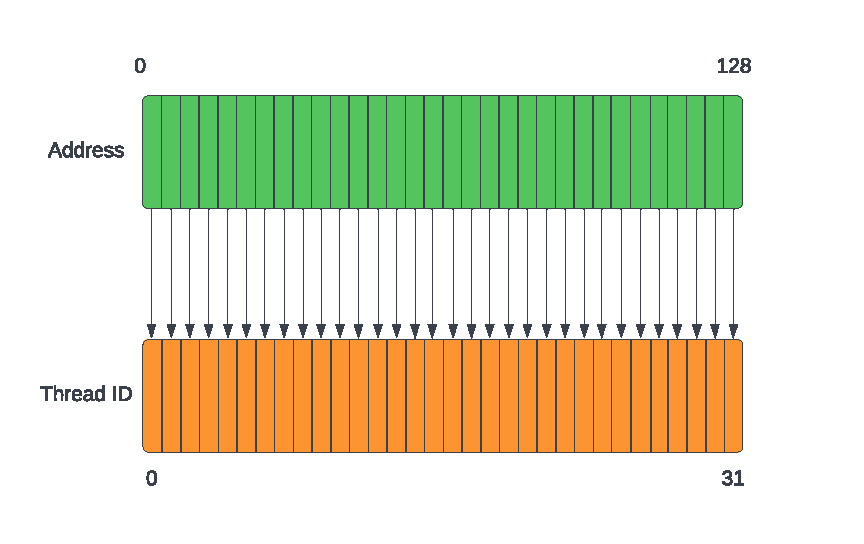
\includegraphics[width=0.8\textwidth]{figures/coalesced access.pdf}
    \caption{Coalesced memory access where a warp of 32 threads loads 128-bytes in a single transaction. Inspired by: https://cvw.cac.cornell.edu/gpu/coalesced}
    \label{fig:coalescedaccess}
\end{figure}

Therefore it is extremely important that we load random variables in a way that minimises the number of transactions (due to the much slower global memory). If we were to arrange the accesses such that each thread were to load $N$ contiguous random variables from memory during path simulation, at each step we would have to sequentially perform a separate memory transaction for each thread. This can incur costs of a lot more than 10x when compared to coalesced accesses. As such, we access random variables such that a single transaction satisfies a whole warp.


To perform path generation, we use two types of random number generator from cuRAND: \texttt{CURAND_RNG_PSEUDO_DEFAULT} and \texttt{CURAND_RNG_QUASI_SCRAMBLED_SOBOL32}. Due to the nature of low-discrepancy sequences we must specify a dimension for the Sobol' generator, we use the number of timesteps in a simulation. We have to pay close attention to the dimensions when using the random variables from the quasi generator as the simulation of each timestep must be independent from each other, thus we must use a random variable from a different dimension. By default, the cuRAND Sobol' generator will output $N/d$ numbers from dimension $1$, followed by $N/d$ from dimension $2$ when generating $N$ variables in $d$ dimensions. The ordering of dimensions is not well spatially-located so we choose to transform the ordering so that coalesced memory access with a smaller stride are possible. Algorithm \ref{alg:QuasiRandomNumbersTransformation} demonstrates this transformation.

\begin{algorithm}[hbt!]
\caption{Transformation of quasi-random variables from $N*\text{PATHS}/d$ of each dimension to BLOCK_SIZE of each dimension repeated, where $N$ is the number of timesteps.}\label{alg:QuasiRandomNumbersTransformation}
\begin{algorithmic}[1]
\State $\text{d_z[PATHS*N]}$ \Comment{Output array} 
\State $\text{temp_z[PATHS*N]}$ \Comment{Input array of random numbers}
\State $\text{desired_idx} \gets \text{threadIdx.x} + \text{N} * \text{blockIdx.x} * \text{blockDim.x}$
\State $\text{temp_idx} \gets \text{threadIdx.x} + \text{blockIdx.x} * \text{blockDim.x}$
\For{$i \gets 0..N-1$}
    \State $\text{d_z[desired_idx]} \gets \text{temp_z[temp_idx]}$
    \State $\text{desired_idx} \gets \text{desired_idx} + \text{blockDim.x}$
    \State $\text{temp_idx} \gets \text{temp_idx} + \text{PATHS}$
\EndFor
\end{algorithmic}
\end{algorithm}

Shown in in Figure \ref{fig:QuasiVariableTransformation} is the input and output ordering of random variables. We see that $B$ variables, where $B$ is BLOCK\_DIM, are taken from each dimension and placed next to each other. This process is repeated such that we have PATHS sets of random numbers from dimension $1$ to $d$. One set will be used by one block such that the BLOCK\_SIZE threads in that block simulate a single path each (one timestep uses one of the dimensions), with the random variable accesses being coalesced.

\begin{figure}[h]
    \centering
    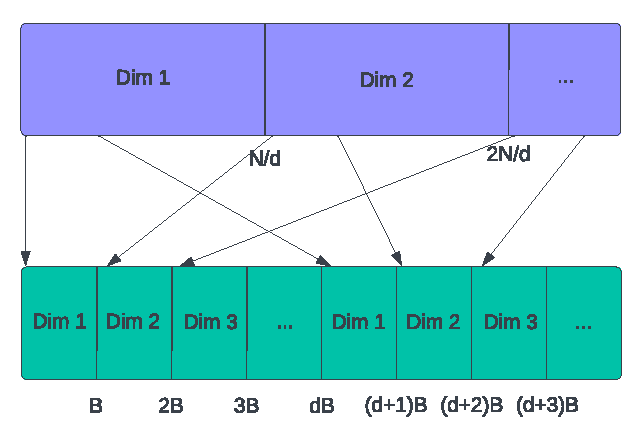
\includegraphics[width=0.7\textwidth]{figures/quasi ordering transform.pdf}
    \caption{Transformation of cuRAND Sobol' numbers from input (top) to output (bottom) ordering.}
    \label{fig:QuasiVariableTransformation}
\end{figure}

In order to reduce the memory footprint and number of accesses, the results of path simulation are not stored for standard MC and standard QMC and required results are calculated on-the-fly during path simulation. This decision also reinforces the decision to encapsulate simulation inside of each product - discussed in \ref{sec:Products}. This allows us to store values required for calculation of the Greeks (such as $S_A$) whilst simulating the path, and use them in the later steps. The basic steps are outlined in Algorithm \ref{alg:PathSimulation}. The separation of $S$ and $\widetilde{S}$ is necessary so that we are able to calculate the Greeks estimates as per section \ref{sec:qmc-cpwmethod}. For QMC with Brownian bridge construction (see \ref{sec:BBConstructionResults} for futher description) we must store the intermediate Brownian bridge results to consume them for path generation afterwards.

\begin{algorithm}[hbt!]
\caption{Per-thread path simulation where $N$ is the number of simulated timesteps with $dt = 1/N$}\label{alg:PathSimulation}
\begin{algorithmic}[1]
\State $S \gets S_0$
\State $Z \gets \text{RandomNormals[ind]}$
\State $W_1 \gets sqrt(dt) * Z$
\State $\widetilde{W}_1 \gets W_1$
\For{$i \gets 1..N$}
    \State $\text{ind} \gets \text{ind} + \text{blockDim.x}$ \Comment{Coalesced reads, when blockDim.x is a multiple of 32}
    \State $Z \gets \text{RandomNormals[ind]}$
    \State $\widetilde{W}_i \gets \widetilde{W}_i + sqrt(dt) * Z$
    \State $\widetilde{S} \gets S_0 * \exp{(\omega * (n-1)*dt + \sigma * (\widetilde{W} - W_1))}$
    \State $S \gets \widetilde{S} * \exp{(\omega * dt + \sigma * W_1)}$
\EndFor
\end{algorithmic}
\end{algorithm}

\section{Products} \label{sec:Products}
It is required to calculate the prices and sensitivities of a variety of options and the functions to do so typically vary between different option types. However, the overall process is the same for pricing any derivative, namely: simulate paths of the underlying asset, followed by calculating the prices and Greeks given the simulated path. These two requirements are that of any option and as such we combine them into a \textit{product}. In this paper we focus on three types of exotic option: arithmetic Asian, binary Asian and lookback. For derivations of the Greek estimates as in \ref{sec:qmc-cpwmethod} see section \ref{sec:GreeksCalculation}. Each of these products implements its own path simulation and Greeks calculation method.

Inheritance and virtual functions are widely-used in standard C++ and similar programming languages, however there are many more restrictions with CUDA. Due to having separate address spaces, copying objects with virtual functions from host memory to device memory can be tricky. To avoid unnecessary complexity, we avoid the use of inheritance directly in kernels (on device) and use them only to aid readability and development. To avoid inheritance directly, we make use of templating in C++. That is, kernels which are used for multiple option types are templated so that at compile time distinct versions of the kernel are generated for each option. From this we obtain the same benefits from inheritance such as minimal repetition of code, without having to copy objects with virtual function tables across address spaces or perform any casts. 

Each thread instantiates its own local copy of the product which has member fields for values such as the underlying's price at the current timestep, running averages, and index to the current random variable. The \textit{SimulatePath} method is called and that thread performs a single simulation for the product, calculating any intermediate values such as the average underlying price or the inner sum of the vega estimate. The final call is to the \textit{CalculatePayoffs} function which calculates the price of the option and Greeks, then places these values back into the global struct of arrays of results.

\section{Antithetic variables}
As a variance reduction technique we have used antithetic variables as described in \ref{sec:antitheticvariables}. Using the already generated random normal variables for the standard MC simulation, we take their complement and simulate a second path from which another set of estimates are calculated. The estimates from the standard and antithetic paths can then be combined to produce the variance reduced final estimate. Adding antithetic variables requires minimal storage on device as we only need to add fields to our products struct that represent the antithetic counterpart to the standard MC values such as $\widetilde{S}(t_j)$.

\section{Brownian bridge construction} \label{sec:BBConstructionResults}
For QMC, we have implemented Brownian bridge construction as a variance reduction method. As shown in Algorithm \ref{alg:PathSimulation} we generate the Brownian motion $\widetilde{W}_i$ from left to right (i.e. from $i=1\dots,d$). However, we may choose to generate the $\widetilde{W}_i$ in any order as long as we sample from the correct conditional distribution given the values already generated. Conditioning a Brownian motion on its endpoints produces a \textit{Brownian bridge} \cite{glasserman2004monte}. The basic idea is that we generate the final value $\widetilde{W}_d$, then continue to fill in each intermediate value: $\widetilde{W}_{d/2}$, then $\widetilde{W}_{d/4}$ and $\widetilde{W}_{3d/4}$ etc, until all values are calculated. For further explanation of how the conditional mean and variance are derived, the reader is referred to section 3.1 of \cite{glasserman2004monte}.

Our implementation does not construct the path directly using a Brownian bridge, but rather uses the bridge to calculate the increments in the path. This allows us to construct $\widetilde{W}$ simply by iterating through the output of the Brownian bridge construction and adding it to the previous value. Algorithm \ref{alg:BrownianBridgeConstruction} demonstrates the process of constructing the Brownian bridge increments.

\begin{algorithm}[hbt!]
\caption{Construction of Brownian bridge increments where the number of timesteps is equal to $2^m$. \textit{idx_zero} is passed to each thread as the first index into the global path array.}\label{alg:BrownianBridgeConstruction}
\begin{algorithmic}[1]
\State $\text{path[idx_zero]} \gets \text{d_z[idx]}$ \Comment{Put first random variable (representing terminal value) in path}
\For{$k \gets 1..m$}
    \State $i \gets 2^k - 1$
    \For{$j \gets 2^{k-1}-1..0$}
        \State $\text{idx} \gets \text{idx} + \text{blockDim.x}$ \Comment{Access next random variable}
        \State $z = \text{d_z[idx]}$
        \State $a \gets 0.5 * \text{path[idx_zero} + j * \text{blockDim.x]}$
        \State $b \gets \sqrt{1 / 2^{k+1}}$
        \State $\text{path[idx_zero} + i * \text{blockDim.x]} \gets a - b * z$
        \State $i \gets i - 1$
        \State $\text{path[idx_zero} + i * \text{blockDim.x]} \gets a + b * z$
        \State $i \gets i - 1$
    \EndFor
\EndFor
\end{algorithmic}
\end{algorithm}

Brownian bridge construction gives finer control over the overall structure of the simulated path as opposed to the standard recursion technique: we use only one random variable to generate the terminal value and then continue to add more and more detail to the rest of the path. Furthermore, when using Sobol' sequences, the first random variables are particularly well distributed leading to the terminal values also being well distributed. This is due to the fact that the initial coordinates of a Sobol' sequence have superior uniformity to that of higher-indexed coordinates \cite{glasserman2004monte}. As the terminal value is often more important than other values in the path this can lead to less error in the estimates produced by Brownian bridge construction with Sobol' sequences. An example of how the path is generated as more points are sampled can be seen in Figure \ref{fig:BrownianBridgePlots}.

The main downside with performing Brownian bridge construction rather than the standard approach is that we need to store the generated path to later consume to simulate the stock price in the variable separated form as per \ref{sec:VariableSeparationPathSimulation}. This means we not only use more global memory on device but will also have a slower kernel runtime due to the increase in memory accesses. However, with this trade-off we expect to achieve a much smaller error in our estimates.

\begin{figure}[h]
    \centering
    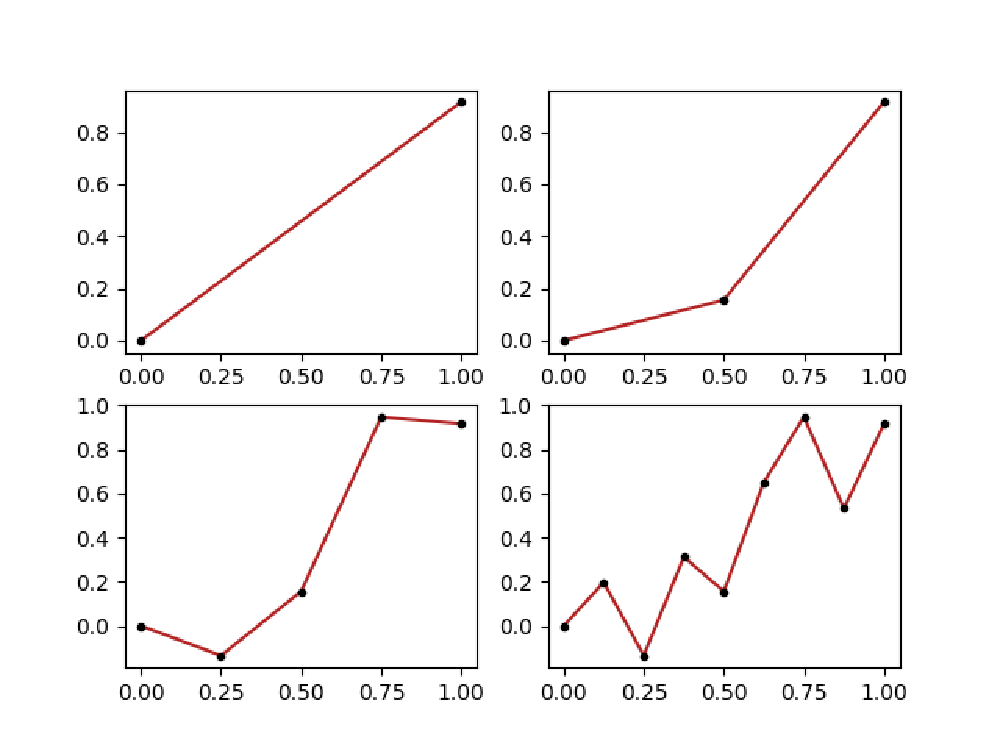
\includegraphics[width=0.8\textwidth]{figures/bb construction.pdf}
    \caption{Brownian bridge construction after $1$, $2$, $4$ and $8$ points have been sampled conditional on the previous values generated.}
    \label{fig:BrownianBridgePlots}
\end{figure}

\section{Greeks calculation} \label{sec:GreeksCalculation}
The step of calculating Greeks is actually quite straightforward. Once we have simulated the path and saved the required values we simply need to evaluate the estimates and store them. Below we list the derived Greeks that are used to calculate estimates as per \cite{ZhangConditionalQuasiMonteCarloMethod} following on from the example in \ref{sec:BaDeltaExample}.

\subsection{Binary Asian Greeks}
As we have already shown the full derivation for the delta, we continue with the estimates for gamma and vega.

\begin{equation*}
\begin{aligned}
    gamma: \frac{{\partial}^2 G}{\partial {S(0)}^2} &= \frac{e^{-rT}}{{S(0)}^2\sigma \sqrt{t_1}}\phi(\psi_d)\left(\frac{\psi_d}{\sigma \sqrt{t_1}} - 1\right). \\[10pt]
\end{aligned}
\end{equation*}

\begin{equation*}
\begin{aligned}
    vega: \frac{{\partial}^2 G}{\partial \sigma} &= e^{-rT}\phi(\psi_d) \left[ \frac{1}{d\sigma \sqrt{t_1}\widetilde{S}_A} \sum_{j=1}^d{\widetilde{S}(t_j) (\widetilde{B}(t_j - t_1) - \sigma(t_j - t_1))} + \frac{\psi_d}{\sigma} - \sqrt{t_1} \right]. \\[10pt]
\end{aligned}
\end{equation*}

Note that the sum inside of the vega calculation is an example of one of the values that is calculated on-the-fly during the path simulation, allowing us to disregard storing the path for standard MC and QMC and storing single precision values only.

\subsection{Arithmetic Asian Greeks}
By taking the conditional expectation we obtain the smoothed payoff

\begin{equation*}
    G(\theta, \boldsymbol{z}) = e^{r(t_1 - T)} \widetilde{S}_A \left[1 - \Phi(\psi_d - \sigma \sqrt{t_1} \right] - e^{-rT}K\left[ 1 - \Phi(\psi_d) \right]
\end{equation*}

We can now differentiate with respect to our parameters of interest to obtain the following estimates.

\begin{equation*}
\begin{aligned}
    delta: \frac{\partial G}{\partial {S(0)}} &= e^{r(t_1 - T)} \frac{\widetilde{S}_A}{S(0)}\left[1 - \Phi(\psi_d - \sigma \sqrt{t_1}) \right]. \\[10pt]
\end{aligned}
\end{equation*}

\begin{equation*}
\begin{aligned}
    gamma: \frac{{\partial}^2 G}{\partial {S(0)}^2} &= \frac{Ke^{-rT}}{{S(0)}^2\sigma\sqrt{t_1}} \phi(\psi_d). \\[10pt]
\end{aligned}
\end{equation*}

\begin{equation*}
\begin{aligned}
    vega: \frac{{\partial} G}{\partial \sigma} &= e^{r(t_1 - T)} \left[1 - \Phi(\psi_d - \sigma \sqrt{t_1}) \right] \frac{1}{d}\sum_{j=1}^d{\widetilde{S}(t_j) (\widetilde{B}(t_j - t_1) - \sigma(t_j - t_1))} + Ke^{-rT}\phi(\psi_d)\sqrt{t_1}. \\[10pt]
\end{aligned}
\end{equation*}

\subsection{Lookback Greeks}
Again, we take the conditional expectation to obtain the smoothed payoff

\begin{equation*}
    G(\theta, \boldsymbol{z}) = e^{r(t_1 - T)} \widetilde{S}_{max} \left[1 - \Phi(\psi_d - \sigma \sqrt{t_1} \right] - e^{-rT}K\left[ 1 - \Phi(\psi_d) \right],
\end{equation*}

where $\widetilde{S}_{max}$ is the maximum value of $\widetilde{S}(t_j)$ for $j = 1,\dots,d$, and $\psi_d = (\ln{K} - \ln{\widetilde{S}_{max}} - \omega t_1) / \sigma \sqrt{t_1}$. By taking differentiation with respect to our parameters we obtain the estimates

\begin{equation*}
\begin{aligned}
    delta: \frac{\partial G}{\partial {S(0)}} &= e^{r(t_1 - T)} \frac{\widetilde{S}_{max}}{S(0)}\left[1 - \Phi(\psi_d - \sigma \sqrt{t_1}) \right]. \\[10pt]
\end{aligned}
\end{equation*}

\begin{equation*}
\begin{aligned}
    gamma: \frac{{\partial}^2 G}{\partial {S(0)}^2} &= \frac{Ke^{-rT}}{{S(0)}^2\sigma\sqrt{t_1}} \phi(\psi_d). \\[10pt]
\end{aligned}
\end{equation*}

\begin{equation*}
\begin{aligned}
    vega: \frac{{\partial} G}{\partial \sigma} &= e^{r(t_1 - T)} \left[1 - \Phi(\psi_d - \sigma \sqrt{t_1}) \right] \frac{1}{d}\sum_{j=1}^d{\widetilde{S}(t_j) (\widetilde{B}(t_j - t_1) - \sigma(t_j - t_1)) \boldsymbol{1}\{\widetilde{S}(t_j) = \widetilde{S}_{max}\}}\\ 
    &\quad + Ke^{-rT}\phi(\psi_d)\sqrt{t_1}. \\[10pt]
\end{aligned}
\end{equation*}

\section{Likelihood Ratio estimates}
As a baseline for the error in the Greek estimates, we implement the LR method through Monte Carlo simulation. Taking the ideas in \ref{sec:LikelihoodRatioMethod} we apply LR to our set of options. The expression given in (\ref{eqn:LRUnbiasedEstimate}) shows that

\begin{equation*}
    f(X) \frac{g^\prime_\theta(X)}{g_\theta(X)},
\end{equation*}

is an unbiased estimator of the derivative of $E[Y]$ with respect to parameter $\theta$. The expression $g^\prime_\theta(X)/g_\theta(X)$ is commonly referred to as the \textit{score}. Calculating Greeks using LR simplifies to calculating the product of the discounted payoff and the relevant score for the Greek. 

Below are listed the scores for the Greeks of each of the three options we are concerned with.

\begin{equation*}
\begin{aligned}
    delta: \frac{Z_1}{S(0)\sigma\sqrt{t_1}}. \\[10pt]
\end{aligned}
\end{equation*}
\begin{equation*}
\begin{aligned}
    gamma: \frac{Z_1^2 - 1}{{S(0)}^2 \sigma^2 t_1} - \frac{Z_1}{{S(0)}^2 \sigma \sqrt{t_1}}. \\[10pt]
\end{aligned}
\end{equation*}
\begin{equation*}
\begin{aligned}
    vega: \sum_{j=1}^d{\frac{Z_j^2 - 1}{\sigma} - Z_j\sqrt{t_1}}. \\[10pt]
\end{aligned}
\end{equation*}

Note that the scores for the three options are equal and the difference between the estimates is simply the form of the payoff.

\section{CPU implementation}
To demonstrate the superior speed when using GPUs we implement a naive, sequential Monte Carlo simulation with the same form of estimates from the aforementioned sections. The implementation has the general form shown in Algorithm \ref{alg:EstimateExpectedPayoff}. The random normal variables generated for use in the GPU simulation are reused by the CPU simulation, in which a single thread performs \textit{NPATH} simulations of $N$ timesteps each. After each path simulation the estimates are calculated and stored in the results struct in the same way that a single GPU thread does.

\chapter{Results} \label{cha:Results}
To demonstrate the effectiveness of the QMC-CPW method from section \ref{sec:qmc-cpwmethod} we run many simulations on the GPU and calculate the variance reduction factors (VRFs) for multiple methods. Using the Likelihood Ratio estimate as the baseline for variance, the VRF for a method is calculated as 

\begin{equation*}
    \frac{\sigma^2_0}{\sigma^2},
\end{equation*}

where $\sigma^2_0$ is the variance in the LR estimate for the Greek. For all methods the estimates for the Greeks are calculated over $P$ number of paths of $N$ timesteps, such that the estimate from a single path is given as

\begin{equation*}
    C^{(\ell)} = {F(\theta,\boldsymbol{z}_\ell}),
\end{equation*}

where $\boldsymbol{z}_\ell$ is a vector of $N$ normal random variables and $F(\theta, x)$ is the underlying function we wish to estimate (e.g. the delta estimate for an arithmetic Asian option). To calculate the error in the estimate we perform $L$ independent runs of the simulation with $P$ fixed such that the final estimate is given as

\begin{equation*}
    C = \frac{1}{L} \sum_{\ell=1}^{L} C_P^{(\ell)},
\end{equation*}

where $C_P^{(\ell)}$ is the estimate from the $\ell$th run over $P$ paths. Finally, the error in the estimate is calculated as follows:

\begin{equation*}
    \sigma = \sqrt{\frac{1}{L} \sum_{\ell=1}^{L} {(C - C_P^{(\ell)})}^2}.
\end{equation*}

For delta, gamma and vega estimation we compare four methods: standard Monte Carlo with CPW estimates (MC-CPW), Monte Carlo with antithetic variables and CPW estimates (MC+AV-CPW), Quasi-Monte Carlo with CPW estimates (QMC-CPW), and finally Quasi-Monte Carlo with Brownian bridge construction and CPW estimates (QMC+BB-CPW). Following a similar style as in \cite{ZhangConditionalQuasiMonteCarloMethod} we perform the simulations over a range of strike prices $K=90,100,110$, and two values for the number of discrete time steps $d=64,256$. We denote the option as "in the money" at $K=90$, "at the money" at $K=100$ and "out the money" at $K=110$. The number of paths, initial stock price, volatility, and risk-free interest rate are all constant and equal for each option type with $P = 2^{15}$,  $S(0) = 100$, $\sigma = 0.2$, and $r = 0.1$. The expiration date for each option $T = 1.0$, or one year. We perform $L=500$ independent runs for all methods. The VRFs for arithmetic, binary and lookback options are presented in tables \ref{tbl:vrfs-arithmetic}-\ref{tbl:vrfs-lookback} respectively. Later we discuss the behaviour of the error in Greek estimates as we increase the number of path simulations per independent run. Information about the \textit{Tesla T4} GPU and the specifications of the CUDA toolkit that was used to collect the results can be found in Appendix \ref{app:gpu-cuda-specs}.

We can make the following observations from the experimental results:

\begin{itemize}
    \item The QMC+BB-CPW method is the most accurate in almost all cases. This is due to the combination of the CPW method which smooths the integrand, allowing for QMC method to work more efficiently, and the Brownian bridge construction which further reduces variance through the methods described in section \ref{sec:BBConstructionResults}.
    \item For the arithmetic Asian option we see QMC+BB-CPW as the best method in all experiments, with VRFs in the hundreds of thousands, and in many cases more than $10$x accurate in comparison to QMC-CPW and MC+AV-CPW. When looking at the VRFs for gamma estimates of the arithmetic Asian option (Table \ref{tbl:vrfs-arithmetic}), MC+AV-CPW outperforms QMC-CPW and this could be due to MV+AV-CPW effectively simulating twice as many paths (standard + antithetic paths) which of course helps to reduce the variance. However, this is not the case for the delta and vega estimates which is interesting to note.
    \item Strike price does affect the performance of many experiments, particularly for the delta and gamma estimates, in which we see an increase in the strike leading to a decrease in VRF.
    \item We discuss dimensionality later, but it also has an effect on the accuracy and becomes more apparent for QMC methods.
\end{itemize}

\begin{table}[!h]
\centering
$\begin{array}{ c c c c c c c c } 
 \hline
 \text{Greeks} & K & d & \text{LR+MC} & \text{MC-CPW} & \text{MC+AV-CPW} & \text{QMC-CPW} & \text{QMC+BB-CPW} \\
 \hline
 \text{delta} & 90  & 64  & 1 & 623     & 3{,}209 & 5,784    & \boldsymbol{154{,}860} \\ 
              &     & 256 & 1 & 2{,}159 & 9{,}527 & 11{,}976 & \boldsymbol{106{,}806} \\
              & 100 & 64  & 1 & 106     & 963     & 903      & \boldsymbol{52{,}689} \\
              &     & 256 & 1 & 353     & 2{,}702 & 1{,}735  & \boldsymbol{34{,}478} \\
              & 110 & 64  & 1 & 35      & 172     & 207      & \boldsymbol{13{,}226} \\
              &     & 256 & 1 & 103     & 423     & 445      & \boldsymbol{7{,}645} \\
 \\
 \text{vega} & 90  & 64  & 1 & 471     & 1{,}566 & 14,603   & \boldsymbol{442{,}513} \\ 
             &     & 256 & 1 & 1{,}595 & 5{,}424 & 30{,}894 & \boldsymbol{340{,}858} \\
             & 100 & 64  & 1 & 294     & 759     & 7{,}770  & \boldsymbol{376{,}285} \\
             &     & 256 & 1 & 967     & 2{,}540 & 18{,}162 & \boldsymbol{633{,}051} \\
             & 110 & 64  & 1 & 113     & 289     & 3{,}195  & \boldsymbol{119{,}816} \\
             &     & 256 & 1 & 330     & 917     & 6{,}701  & \boldsymbol{294{,}813} \\
 \\
 \text{gamma} & 90  & 64  & 1 & 20{,}393  & 49{,}141  & 28{,}067  & \boldsymbol{271{,}351} \\ 
              &     & 256 & 1 & 108{,}667 & 275{,}370 & 134{,}644 & \boldsymbol{487{,}940} \\
              & 100 & 64  & 1 & 3{,}814   & 9{,}433   & 5{,}427   & \boldsymbol{75{,}020} \\
              &     & 256 & 1 & 20{,}967  & 49{,}834  & 21{,}116  & \boldsymbol{72{,}558} \\
              & 110 & 64  & 1 & 1{,}101   & 2{,}468   & 1{,}477   & \boldsymbol{23{,}085} \\
              &     & 256 & 1 & 5{,}977   & 13{,}770  & 6{,}147   & \boldsymbol{25{,}695} \\
 \hline
\end{array}$
\caption{VRFs for arithmetic Asian option on GPU with $2^{15}$ paths. $S(0) = 100$, $\sigma = 0.2$, $r = 0.1$ and $T = 1$.}
\label{tbl:vrfs-arithmetic}
\end{table}

\begin{itemize}
    \item For delta and vega estimates of the binary Asian option (Table \ref{tbl:vrfs-binary}) we see QMC+BB-CPW outperforming all other methods and taking advantage of the increased smoothness of the integrand.
    \item We see little or no improvement of QMC-CPW over MC-CPW for all estimates of the binary option which could be an indication of the limitations of QMC in high dimensions.
    \item We also see this in the gamma estimates for the binary Asian option, where even QMC+BB-CPW is outperformed by MC+AV-CPW for all of the experiments with $256$ timesteps. A technique to reduce the effective dimension of the problem such as Principle Component Analysis (PCA) would likely remove these differences and result in a substantial decrease in error for the QMC methods.
    \item The binary Asian option results in some of the smallest VRFs for all Greek estimates especially for the delta and gamma.
    \item Again, we see the strike price having a large impact on the VRFs. For example the delta estimate with $K=90$ over $256$ timesteps in Table \ref{tbl:vrfs-binary} is $714$ and decreases to $150$ for $K=110$.
\end{itemize}

\begin{table}[!h]
\centering
$\begin{array}{ c c c c c c c c } 
 \hline
 \text{Greeks} & K & d & \text{LR+MC} & \text{MC-CPW} & \text{MC+AV-CPW} & \text{QMC-CPW} & \text{QMC+BB-CPW} \\
 \hline
 \text{delta} & 90  & 64  & 1 & 109 & 247 & 150 & \boldsymbol{1{,}447} \\ 
              &     & 256 & 1 & 159 & 389 & 197 & \boldsymbol{714} \\
              & 100 & 64  & 1 & 43  & 123 & 58  & \boldsymbol{830} \\
              &     & 256 & 1 & 64  & 150 & 64  & \boldsymbol{221} \\
              & 110 & 64  & 1 & 23  & 69  & 32  & \boldsymbol{497} \\
              &     & 256 & 1 & 35  & 89  & 36  & \boldsymbol{150} \\
 \\
 \text{vega} & 90  & 64  & 1 & 326     & 733     & 447     & \boldsymbol{4{,}227} \\ 
             &     & 256 & 1 & 481     & 1{,}168 & 593     & \boldsymbol{2{,}114} \\
             & 100 & 64  & 1 & 771     & 2{,}078 & 1{,}176 & \boldsymbol{12{,}571} \\
             &     & 256 & 1 & 1{,}419 & 3{,}405 & 1{,}502 & \boldsymbol{5{,}111} \\
             & 110 & 64  & 1 & 839     & 1{,}965 & 1{,}167 & \boldsymbol{9{,}232} \\
             &     & 256 & 1 & 1{,}976 & 4{,}617 & 1{,}950 & \boldsymbol{7{,}803} \\
 \\
 \text{gamma} & 90  & 64  & 1 & 363 & 713                  & 376 & \boldsymbol{999} \\ 
              &     & 256 & 1 & 691 & \boldsymbol{1{,}446} & 673 & 883 \\
              & 100 & 64  & 1 & 136 & 201                  & 126 & \boldsymbol{784} \\
              &     & 256 & 1 & 201 & \boldsymbol{415}     & 212 & 392 \\
              & 110 & 64  & 1 & 79  & 137                  & 67  & \boldsymbol{355} \\
              &     & 256 & 1 & 116 & \boldsymbol{237}     & 117 & 179 \\
 \hline
\end{array}$
\caption{VRFs for binary Asian option on GPU with $2^{15}$ paths. $S(0) = 100$, $\sigma = 0.2$, $r = 0.1$ and $T = 1$.}
\label{tbl:vrfs-binary}
\end{table}

\begin{table}[H]
\centering
$\begin{array}{ c c c c c c c c } 
 \hline
 \text{Greeks} & K & d & \text{LR+MC} & \text{MC-CPW} & \text{MC+AV-CPW} & \text{QMC-CPW} & \text{QMC+BB-CPW} \\
 \hline
 \text{delta} & 90  & 64  & 1 & 7{,}020  & 58{,}906  & 382{,}145     & \boldsymbol{2{,}631{,}721} \\ 
              &     & 256 & 1 & 26{,}665 & 187{,}898 & 1{,}135{,}848 & \boldsymbol{7{,}737{,}083} \\
              & 100 & 64  & 1 & 1{,}635  & 12{,}183  & 21{,}857      & \boldsymbol{40{,}682} \\
              &     & 256 & 1 & 8{,}323  & 58{,}180  & 79{,}683      & \boldsymbol{171{,}880} \\
              & 110 & 64  & 1 & 233      & 1{,}899   & 1{,}896       & \boldsymbol{13{,}181} \\
              &     & 256 & 1 & 920      & 5{,}594   & 4{,}264       & \boldsymbol{23{,}354} \\
 \\
 \text{vega} & 90  & 64  & 1 & 501     & 2{,}333 & 10{,}667 & \boldsymbol{51{,}816} \\ 
             &     & 256 & 1 & 1{,}855 & 7{,}492 & 33{,}043 & \boldsymbol{165{,}179} \\
             & 100 & 64  & 1 & 311     & 1{,}420 & 6{,}580  & \boldsymbol{35{,}370} \\
             &     & 256 & 1 & 1{,}138 & 4{,}569 & 20{,}418 & \boldsymbol{103{,}536} \\
             & 110 & 64  & 1 & 178     & 870     & 4{,}601  & \boldsymbol{26{,}065} \\
             &     & 256 & 1 & 657     & 2{,}876 & 13{,}739 & \boldsymbol{69{,}210} \\
 \\
 \text{gamma} & 90  & 64  & 1 & 55{,}102{,}633 & 113{,}383{,}607 & 113{,}193{,}362 & \boldsymbol{129{,}220{,}281} \\ 
              &     & 256 & 1 & 1.2 * 10^{17}  & 4.2 * 10^{17}          & 6.2 * 10^{16}   & \boldsymbol{1.0 * 10^{18}} \\
              & 100 & 64  & 1 & 27{,}235       & 72{,}792               & 89{,}333        & \boldsymbol{212{,}928} \\
              &     & 256 & 1 & 175{,}073      & 393{,}763              & 434{,}423       & \boldsymbol{604{,}285} \\
              & 110 & 64  & 1 & 9{,}787        & 24{,}450               & 13{,}755        & \boldsymbol{42{,}199} \\
              &     & 256 & 1 & 51{,}687       & \boldsymbol{123{,}922} & 60{,}037        & 112{,}398 \\
 \hline
\end{array}$
\caption{VRFs for lookback option on GPU with $2^{15}$ paths. $S(0) = 100$, $\sigma = 0.2$, $r = 0.1$ and $T = 1$.}
\label{tbl:vrfs-lookback}
\end{table}

\begin{itemize}
    \item For the lookback option (Table \ref{tbl:vrfs-lookback}), we see some of the largest VRFs, particularly those for the gamma estimates.
    \item We also see just how great of an effect the strike price has on the lookback option: when $K=90$ and the option is in the money we can see a VRF of $1.0 * 10^{18}$, whereas when the option is at the money and out the money we see estimates in the range of hundreds of thousands.
    \item For the delta and vega estimates QMC-CPW outperforms MC+AV-CPW for almost all experiments, except when $K=110$ for the delta estimate.
\end{itemize}

We also present graphs of the error in Greek estimates over a range of paths. The graphs in Figures \ref{fig:ArithmeticPathErrorsK90}-\ref{fig:LookbackPathErrorsK110} are all calculated over $L=500$ independent runs with $P=2^i$ paths for $i \in [12,19]$, with $256$ timesteps each. The graphs for paths of $64$ timesteps are not included but we see similar behaviour to the graphs presented, and note that the earlier observations about dimensionality for the gamma estimates in table \ref{tbl:vrfs-binary} are maintained. We note the following observations:

\begin{itemize}
    \item QMC+BB-CPW tends to outperform other methods across all numbers of paths.
    \item Its advantage in gamma estimates typically appears to be much smaller except that of the arithmetic Asian option.
    \item For the delta and gamma estimates in Figure \ref{fig:ArithmeticPathErrorsK90} we see QMC-CPW having little or no advantage over MC+AV-CPW.
    \item Vega estimates are typically the least accurate Greek.
    \item As the number of paths approaches $2^{19}$ we begin to see QMC+BB-CPW outperform all other methods for every Greek estimate.
\end{itemize}

\begin{figure}[H]
    \centering
    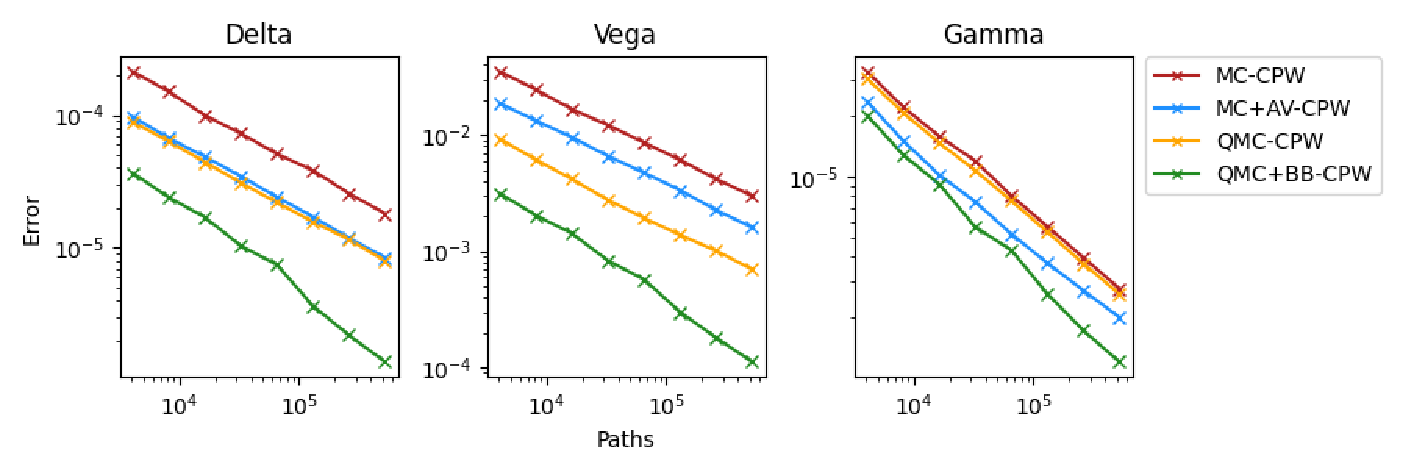
\includegraphics[width=1\textwidth]{figures/arithmetic path errors k=90.pdf}
    \caption{Errors in Greek estimates of an arithmetic Asian option with $S(0)=100$, $K=90$, $\sigma = 0.2$, $r=0.1$, $N=256$, and $T=1$ over $2^{12}$ to $2^{19}$ paths.}
    \label{fig:ArithmeticPathErrorsK90}
\end{figure}

\begin{figure}[H]
    \centering
    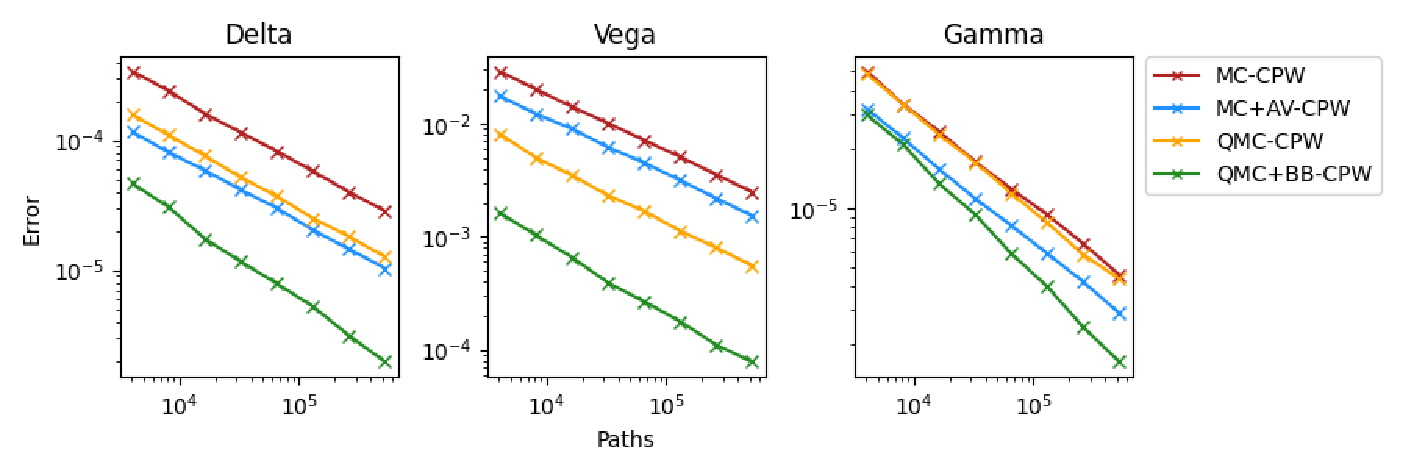
\includegraphics[width=1\textwidth]{figures/arithmetic path errors k=100.pdf}
    \caption{Errors in Greek estimates of an arithmetic Asian option with $S(0)=100$, $K=100$, $\sigma = 0.2$, $r=0.1$, $N=256$, and $T=1$ over $2^{12}$ to $2^{19}$ paths.}
    \label{fig:ArithmeticPathErrorsK100}
\end{figure}

\begin{figure}[H]
    \centering
    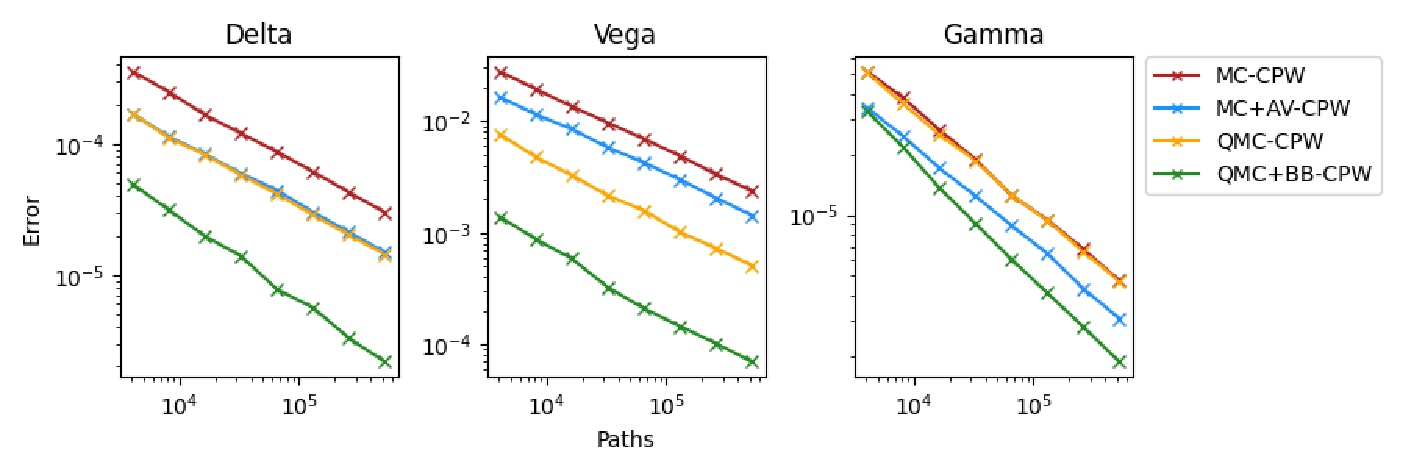
\includegraphics[width=1\textwidth]{figures/arithmetic path errors k=110.pdf}
    \caption{Errors in Greek estimates of an arithmetic Asian option with $S(0)=100$, $K=110$, $\sigma = 0.2$, $r=0.1$, $N=256$, and $T=1$ over $2^{12}$ to $2^{19}$ paths.}
    \label{fig:ArithmeticPathErrorsK110}
\end{figure}

\begin{itemize}
    \item For the arithmetic Asian estimates (figures \ref{fig:ArithmeticPathErrorsK90}-\ref{fig:ArithmeticPathErrorsK110}), QMC+BB-CPW is the best performing method across all number of paths and Greeks.
    \item For gamma estimates in figures \ref{fig:ArithmeticPathErrorsK90}-\ref{fig:ArithmeticPathErrorsK110} the advantage appears to increase as the number of paths increase.
    \item QMC-CPW is greatly outperformed by MC+AV-CPW for the arithmetic option's (figures \ref{fig:ArithmeticPathErrorsK90}-\ref{fig:ArithmeticPathErrorsK110}) gamma estimates of the arithmetic option whilst they perform similarly for delta.
    \item For the first order Greeks (delta and vega in figures \ref{fig:ArithmeticPathErrorsK90}-\ref{fig:ArithmeticPathErrorsK110}) QMC+BB-CPW has a large advantage over the other methods even at a small number of paths. However, for the second order Greek of gamma it's error is roughly equal to that of MC+AV-CPW at a small number of paths and it only gains a noticeable advantage as the number of paths increases.
\end{itemize}

\begin{figure}[H]
    \centering
    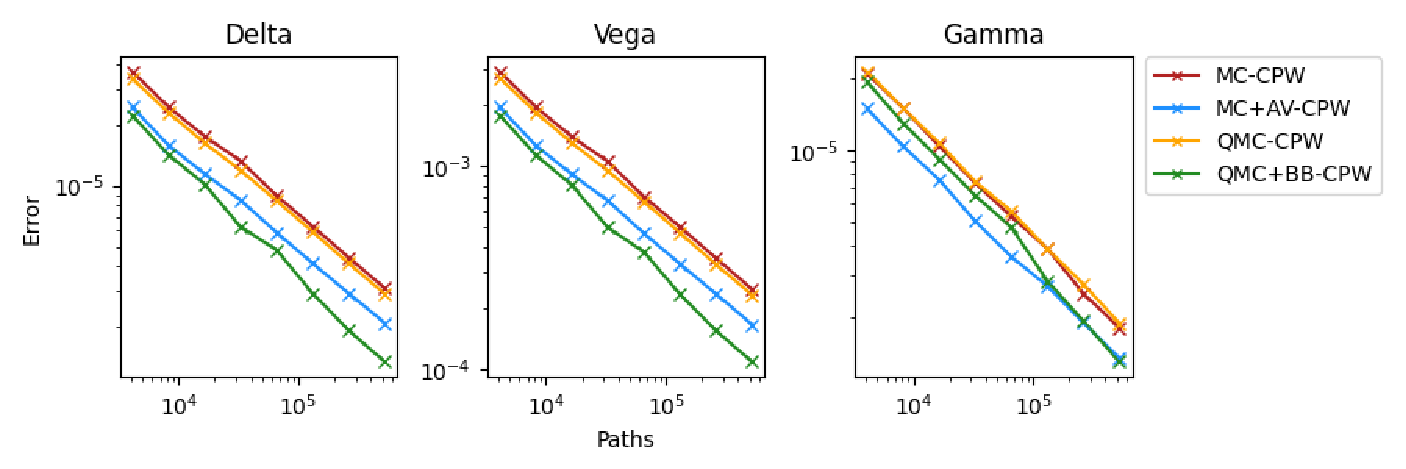
\includegraphics[width=1\textwidth]{figures/binary path errors k=90.pdf}
    \caption{Errors in Greek estimates of a binary Asian option with $S(0)=100$, $K=90$, $\sigma = 0.2$, $r=0.1$, $N=256$, and $T=1$ over $2^{12}$ to $2^{19}$ paths.}
    \label{fig:BinaryPathErrorsK90}
\end{figure}

\begin{figure}[H]
    \centering
    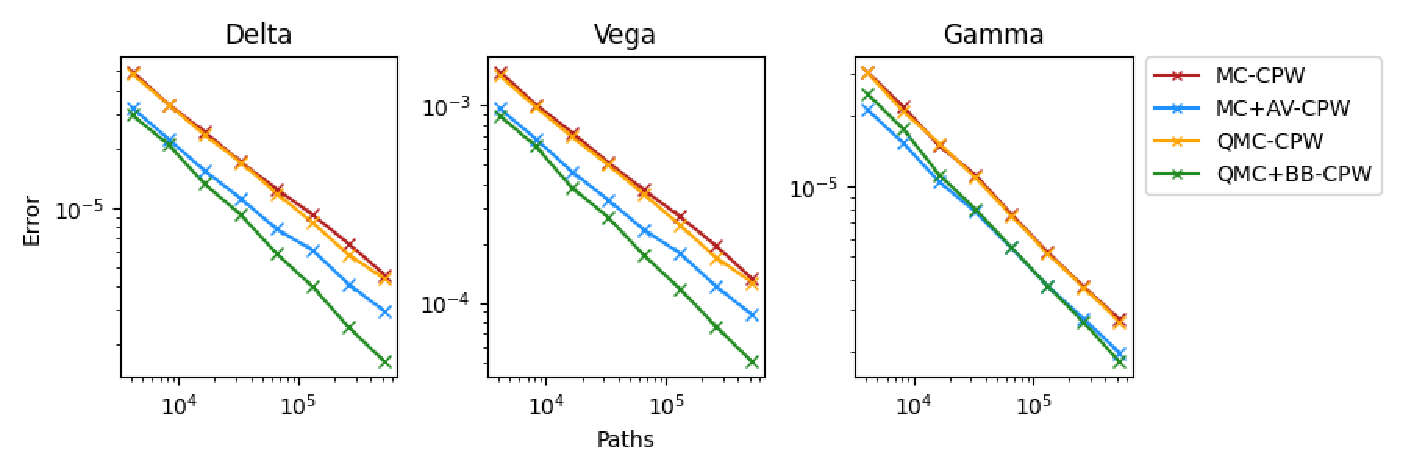
\includegraphics[width=1\textwidth]{figures/binary path errors k=100.pdf}
    \caption{Errors in Greek estimates of a binary Asian option with $S(0)=100$, $K=100$, $\sigma = 0.2$, $r=0.1$, $N=256$, and $T=1$ over $2^{12}$ to $2^{19}$ paths.}
    \label{fig:BinaryPathErrorsK100}
\end{figure}

\begin{figure}[H]
    \centering
    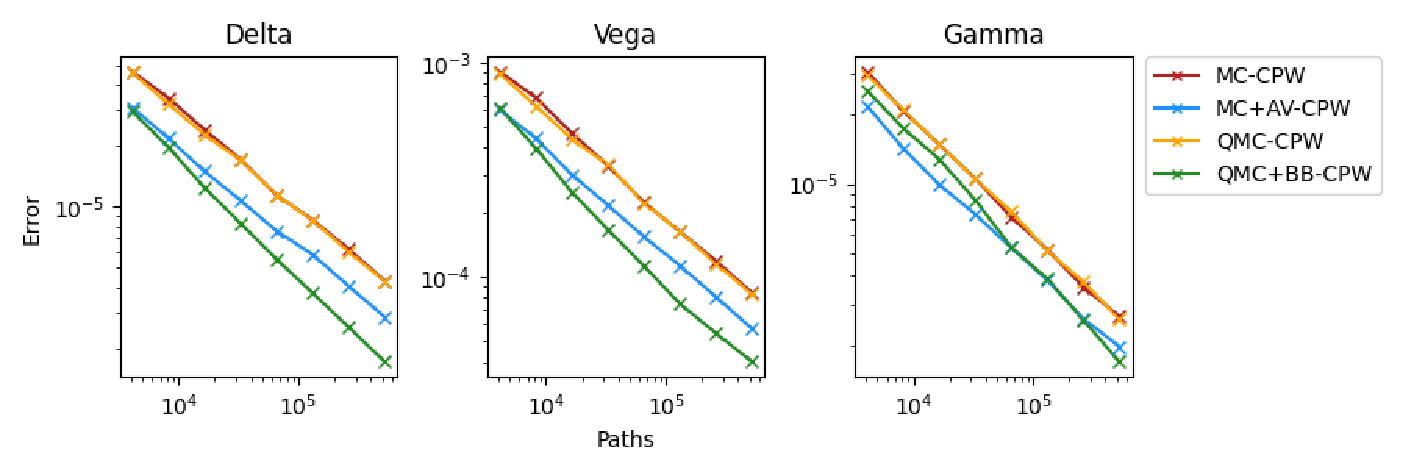
\includegraphics[width=1\textwidth]{figures/binary path errors k=110.pdf}
    \caption{Errors in Greek estimates of a binary Asian option with $S(0)=100$, $K=110$, $\sigma = 0.2$, $r=0.1$, $N=256$, and $T=1$ over $2^{12}$ to $2^{19}$ paths.}
    \label{fig:BinaryPathErrorsK110}
\end{figure}

\begin{itemize}
    \item The errors in the estimates for the binary Asian option (figures \ref{fig:BinaryPathErrorsK90}-\ref{fig:BinaryPathErrorsK110}) are much closer than that of the arithmetic Asian.
    \item For delta and vega of the binary option in figures \ref{fig:BinaryPathErrorsK90}-\ref{fig:BinaryPathErrorsK110}, QMC+BB-CPW is the superior method across all number paths.
    \item MC+AV-CPW tends to match and often outperform QMC+BB-CPW when the number of paths is smaller for the binary option (figures \ref{fig:BinaryPathErrorsK90}-\ref{fig:BinaryPathErrorsK110}). In fact, we only see MC+AV-CPW outperformed for gamma at a very high path number ($2^{19}$).
    \item For all estimates of the binary option (figures \ref{fig:BinaryPathErrorsK90}-\ref{fig:BinaryPathErrorsK110}) we see almost no improvement with QMC-CPW over MC-CPW.
\end{itemize}

\begin{figure}[H]
    \centering
    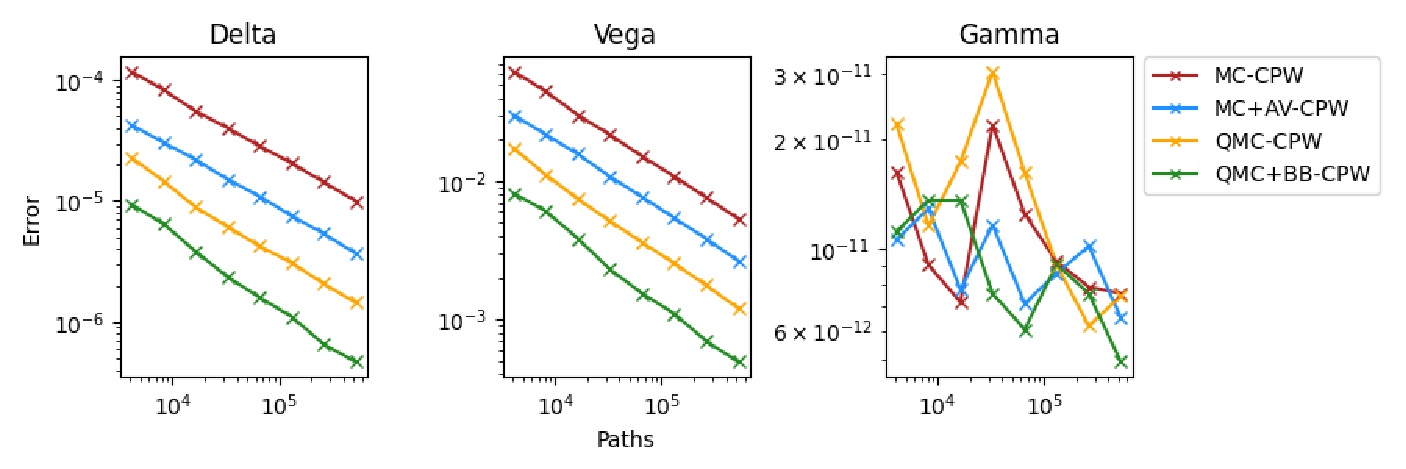
\includegraphics[width=1\textwidth]{figures/lookback path errors k=90.pdf}
    \caption{Errors in Greek estimates of a lookback option with $S(0)=100$, $K=90$, $\sigma = 0.2$, $r=0.1$, $N=256$, and $T=1$ over $2^{12}$ to $2^{19}$ paths.}
    \label{fig:LookbackPathErrorsK90}
\end{figure}

\begin{figure}[H]
    \centering
    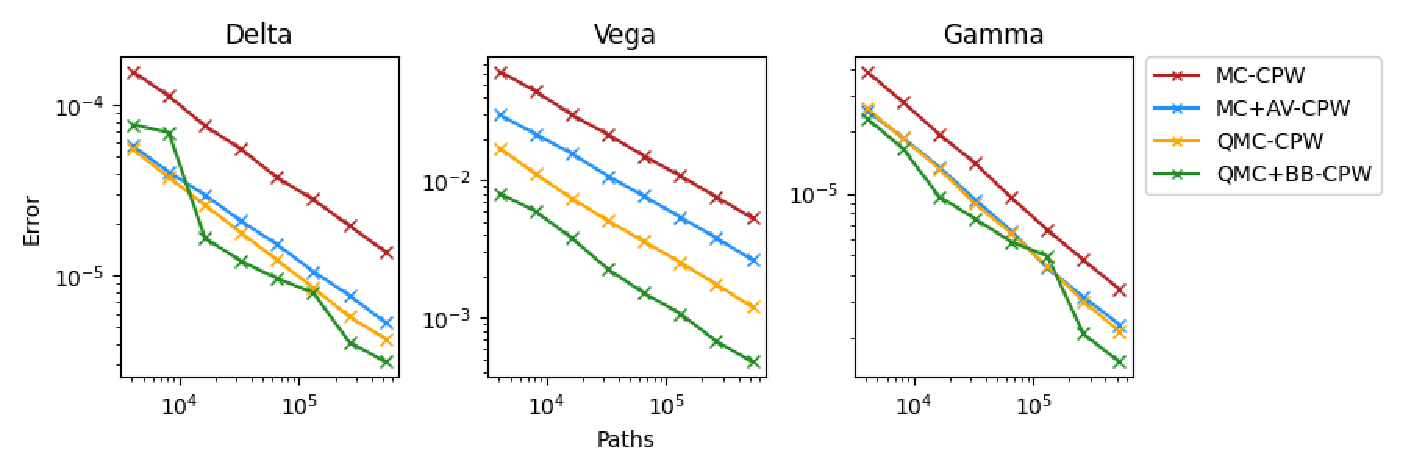
\includegraphics[width=1\textwidth]{figures/lookback path errors k=100.pdf}
    \caption{Errors in Greek estimates of a lookback option with $S(0)=100$, $K=100$, $\sigma = 0.2$, $r=0.1$, $N=256$, and $T=1$ over $2^{12}$ to $2^{19}$ paths.}
    \label{fig:LookbackPathErrorsK100}
\end{figure}

\begin{figure}[H]
    \centering
    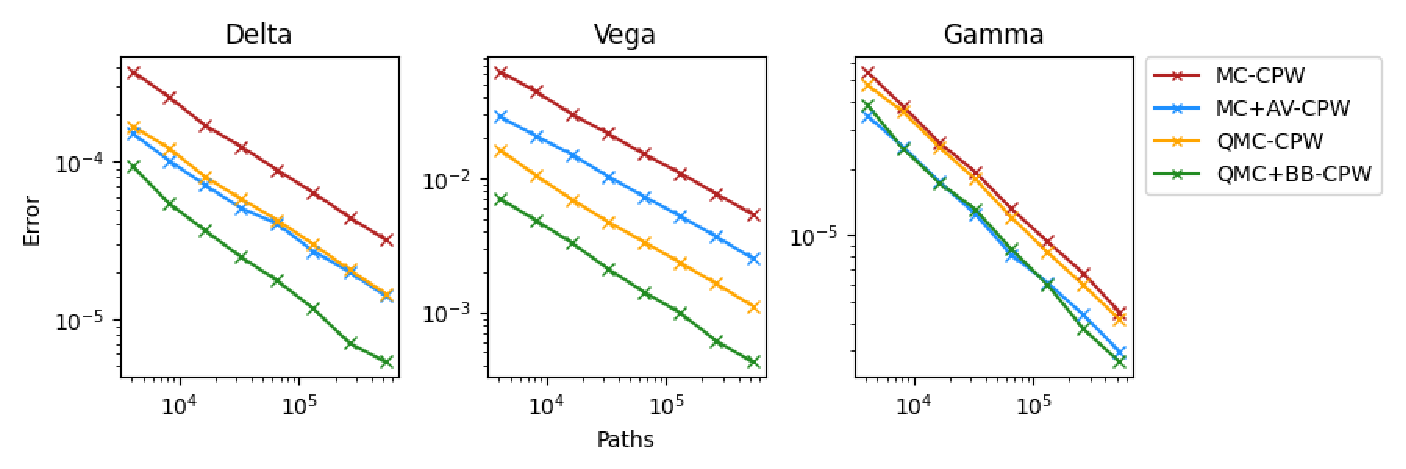
\includegraphics[width=1\textwidth]{figures/lookback path errors k=110.pdf}
    \caption{Errors in Greek estimates of a lookback option with $S(0)=100$, $K=110$, $\sigma = 0.2$, $r=0.1$, $N=256$, and $T=1$ over $2^{12}$ to $2^{19}$ paths.}
    \label{fig:LookbackPathErrorsK110}
\end{figure}

\begin{itemize}
    \item We see the largest variation in performance across the lookback estimates (figures \ref{fig:LookbackPathErrorsK90}-\ref{fig:LookbackPathErrorsK110}).
    \item For the gamma estimates when $K=90$ (in the money, figure \ref{fig:LookbackPathErrorsK90}) the errors are extremely small and don't follow the same monotonically decreasing trend we see in most other graphs.
    \item The vega estimates in figures \ref{fig:LookbackPathErrorsK90}-\ref{fig:LookbackPathErrorsK110} are the most consistent where we see MC-CPW, MC+AV-CPW, QMC-CPW, QMC+BB-CPW as the order from largest error to smallest for $K=90,100,110$.
    \item When the option is at the money in figure \ref{fig:LookbackPathErrorsK100}, we see the least improvement of QMC+BB-CPW over QMC-CPW when compared to other options and estimates, where it is outperformed at a smaller number of paths and even matched at $2^{17}$ paths.
\end{itemize}
 

The final objective was to achieve a significant speed up over a CPU implementation. For the three methods where we do not store the path, we see speedups for a single kernel run when compared to the naive sequential CPU implementation upwards of $500$x for those experiments with $64$ timesteps per path, and upwards of $900$x for those with $256$ timesteps.

The overhead of accessing global memory on device becomes apparent when we see the difference in the speedup between the QMC+BB-CPW experiments and the other methods. Due to having to store the Brownian bridge path construction and then repeatedly accessing the array in global memory we see a significant decrease in speedups from the previously mentioned values to around $200$x for both $64$ and $256$ timesteps. It is interesting to note that the lookback option sees the greatest speed improvement over the CPU.

Although tables \ref{tbl:vrfs-arithmetic}-\ref{tbl:vrfs-lookback} show that MC+AV-CPW outperforms QMC+BB-CPW in some instances, from figures \ref{fig:ArithmeticPathErrorsK90}-\ref{fig:LookbackPathErrorsK110} we see that as the number of paths increases past $2^{15}$, which is the value used for the tables, QMC+BB-CPW tends to become the best performing method.
\chapter{Evaluation} \label{cha:Evaluation}
In this chapter the performance of our implementation is considered, in terms of VRFs and speedups, when compared with other similar solutions.


\section{Performance}
When compared with the implementation by Zhang and Wang \cite{ZhangConditionalQuasiMonteCarloMethod} our most accurate method does not show as large VRFs as theirs. For example, many of their arithmetic Asian delta estimates (ours are in Table \ref{tbl:vrfs-arithmetic}) are in the hundreds of millions whilst ours are in the hundreds of thousands. The implementation difference between this project and that in \cite{ZhangConditionalQuasiMonteCarloMethod} is the variance reduction technique used with QMC. We use the Brownian bridge path construction whereas Zhang and Wang use Gradient Principle Component Analysis (GPCA) \cite{gpca}. Whereas Brownian bridge is most effective for options whose terminal price is considered the most important value (e.g. European options), Asian options do not receive as great a variance reduction due to the form of their payoff. GPCA and PCA has been shown to reduce the effective dimension which makes QMC methods far more efficient, thus Zhang and Wang's implementation sees much better VRFs.

We can directly see the improvement of our implementation over that of the traditional pathwise and likelihood ratio methods simply from Tables \ref{tbl:vrfs-arithmetic}-\ref{tbl:vrfs-lookback}. Noting the significantly better VRFs of QMC+BB-CPW in chapter \ref{cha:Results}, financial institutions would achieve much greater accuracy through the use of our implementation. Given how important calculating Greeks is for these institutions, the benefits from using our implementation are far and wide: a more precise understanding of individual products behaviour to input parameters can allow for a far better understanding of the overall risk a company has to the market. This allows a company to perhaps take on larger positions with more confidence in their exposure and give them the ability to better react to market events. In a more specific situation, having more accurate estimates for Greeks leads to better pricing of products, which can give a market participant an advantage over competitors.

As noted in chapter \ref{cha:Results}, as the number of paths increase, the error in the estimates from QMC+BB-CPW become the smallest of all the methods. We are able to comfortably simulate $2^{19}$ paths on the Tesla T4 GPU, thus the ever-present trade off between speed and accuracy is the main consideration when applying the method. At $2^{15}$ paths (used for tables \ref{tbl:vrfs-arithmetic}-\ref{tbl:vrfs-lookback}) we see a single kernel run take around $0.8$ms for the Brownian bridge construction method and $0.2$ms for the others. The basic CPU implementation at $2^{15}$ paths takes ~$150$ms. As we move up to $2^{19}$ paths, QMC+BB-CPW requires $12$-$13$ms per kernel call and the other methods around $3$ms.

\section{Applicability and design}
Although only applied to three types of option, our method can be implemented for many types of options - both vanilla and exotic. This allows for a single algorithm to be applied to a large set of the products an institution may work with and reduces the need for many distinct methods that depend on the option type, whilst also achieving a higher accuracy. For example, estimating the gamma of many option types is not possible through pathwise alone and so an existing solution would be to apply the likelihood ratio in conjunction with pathwise. Any variant of QMC-CPW is able to calculate gamma estimates so broadens the range of products that an institution can handle with much less overhead.

The templated design of the simulation also allows other option types to be added easily, including those with multiple underlying assets. A redefinition of the path simulation and payoffs/Greeks formula for each type is all that is needed.We are also able to pull out Brownian bridge construction such that products can ingest the increments directly rather than the random normal variables $Z_i$.

One of the current limitations with the design is the lack of dynamic memory allocation, which would allow us to further encapsulate different product types and have a finer-grained control over simulation. In Savine's book \cite{savine2018aad}, a dynamic framework is presented in which options with a varying numbers of required random normal variables for simulation, can all follow the same path through the program. The implementation presented in this report has a fixed number of random numbers to generate at compile time and as such each product is required to take in all of those variables. This design was noted but the added difficulty of dealing with objects containing virtual functions in CUDA was seen as too far aside for the main objective of combining the QMC-CPW method and the parallel performance of the GPU. We recognise that the main objective of this project was experimental results and although added flexibility and a more polished product would be nice to have it was not a key element to begin with. We discuss these points later in section \ref{sec:FutureWork}.
\chapter{Conclusion} \label{cha:Conclusion}
In this project we have presented a powerful method for calculating the Greeks of exotic options on the GPU. The Quasi-Monte Carlo Conditional Pathwise method developed by Zhang and Wang \cite{ZhangConditionalQuasiMonteCarloMethod} allows for smoothing of the integrands which Quasi-Monte Carlo methods take advantage of to efficiently estimate the Greeks. 

Our implementation uses the highly parallel nature of GPUs to efficiently implement the Quasi-Monte Carlo simulation such that our solution is hundreds of times faster than a serial CPU implementation. As a variance reduction technique, Brownian bridge construction is used in conjunction with the CPW estimates to further reduce the error in our Greek estimates. We show that our implementation, QMC+BB-CPW, produces estimates with VRFs in the hundreds of thousands and even up to $1.0 * 10^{18}$ when compared to traditional methods such as the Likelihood Ratio method. When compared to other simulation methods such as MC+AV-CPW, our method outperforms for almost all Greek estimates of arithmetic Asian, binary Asian and lookback options over a range of strike prices.

Whilst the results obtained are more than satisfactory, we do not achieve VRFs of the same magnitude as in \cite{ZhangConditionalQuasiMonteCarloMethod}. This is likely due to their implementation using Gradient Principle Component Analysis as a variance reduction technique which reduces the effective dimension, allowing Quasi-Monte Carlo methods to be even more efficient.

\section{Future work} \label{sec:FutureWork}
There are many possible extensions to the project, from a wide variety of angles. We could implement QMC-CPW for other volatility models such as the Heston model, however this would require a substantial amount of work as the form of all estimates would be vastly different to those presented in this paper. 

A second direct change to the code could be using other random number generation methods. Although we used the built-in cuRAND generators, there is scope to write our own random number generators that are faster than cuRAND's and give us more flexibility in the output ordering and scrambling. 

Both of these changes could be enabled easily by interfacing out the random number generation and volatility models much like our current product implementation.

\subsection{Improved VRFs}
As mentioned earlier, our method does not achieve as large VRFs as we know are possible. To improve this, we could implement further variance reduction techniques such as (Gradient) Principle Component Analysis. Techniques such as this help Quasi-Monte Carlo methods to more efficiently estimate integrals as they are thought to reduce the effective dimension, which in the finance setting can be extremely useful due to the high-dimensionaility of many problems.

\subsection{Producing a polished product}
Moving away from improving the current experimental-style of the project, we could work to build a more polished software solution. This would include some of the previously mentioned improvements such as interfacing out the volatility model and random number generator, but also adding more option types and other financial products. 

Adding more flexibility to the software would also be a key requirement. Spending time researching the best methods for allowing the use dynamic data structures in kernels would be important. Also, the ability to freely, efficiently, and easily move objects from host to device and vice-versa would be very useful. We could attempt to do this through unified memory but could also restrict the software to GPU-only uses whereas we think it is evident that much of the software would be useful for CPU-only programs as well.

An idea for a specific software product would be wrapping our implementation in some networking logic such that it could act as a microservice for calculating Greeks to be used inside of a larger risk-management system. It would receive parameters such as stock price, implied volatility and the expiration dates from the input bus, process these values to produce estimates for Greeks and publish them to other microservices.
\chapter{Ethical Considerations}
This project is largely an experimental demonstration of how a recent method for calculating Greeks can be efficiently implemented on a GPU. We have not had to consider many ethical issues during the development of this project.

However, it is worth noting that all estimates produced by the software can be fully explainable and any errors easily debugged - unlike solutions that come from the neural networks.

Financial exchanges and markets around the world have strict regulations designed to prevent misconduct by participants. This software is not designed, and is highly unlikely, to give any user an unfair, or otherwise illegal, advantage over other market participants.

\bibliographystyle{vancouver}
\bibliography{bibs/bibliography}

\appendix
\chapter{GPU and CUDA specifications} \label{app:gpu-cuda-specs}

CUDA toolkit version 11.2.1 was used for all of the software in this project. The online documentation for this version is available at \href{https://docs.nvidia.com/cuda/archive/11.2.1/}{https://docs.nvidia.com/cuda/archive/11.2.1/}.

All simulations were ran on a single Tesla T4 GPU which has the Turing architecture with compute capability $7.5$. The general information for the device is listed below:

\begin{table}[!h]
\centering
\begin{tabular}{c c}
    \textbf{General Information} & \\
    Name & Tesla T4 \\
    Compute Capability & $7.5$ \\
    Clock Rate (Hz) & $1590000$ \\
    Device Copy Overlap & Enabled \\
    Kernel Execution Timeout & Disabled \\ \\
    \textbf{Memory Information} & \\
    Global Memory & 15843721216 \\
    Constant Memory & 65536 \\
    Max Memory Pitch & 2147483647 \\
    Texture Alignment & 512 \\ \\
    \textbf{Multiprocessor Information} & \\
    Multiprocessor Count & 40 \\
    Shared Memory per MP & 49152 \\
    Registers per MP & 65536 \\
    Threads in Ward & 32 \\
    Max Threads per Block & 1024 \\
    Max Thread Dimensions & (1024, 1024, 64) \\
    Max Grid Dimensions & (2147483647, 65536, 65535) \\
\end{tabular}
\caption{Tesla T4 specifications. Memory values are given in bytes.}
\label{tbl:TeslaT4Specs}
\end{table}

\end{document}